\documentclass[conference]{IEEEtran}
\IEEEoverridecommandlockouts
\usepackage[T1]{fontenc}
\usepackage{lmodern}
\usepackage{cite}
\usepackage{amsmath,amssymb}
\usepackage{graphicx}
\usepackage{booktabs}
\usepackage{array}
\usepackage{adjustbox}
\usepackage{multirow}
\usepackage{xcolor}
\usepackage{url}
\usepackage{tikz}
\usetikzlibrary{arrows.meta,positioning}
\usepackage[hidelinks]{hyperref}

\newcommand{\pp}{\,pts}
\newcommand{\repourl}{https://github.com/REPLACE/hit-song-prediction}

\begin{document}

\title{What Really Predicts a Hit?\\ Artist History, Era Context and Shortcut Features\\ in Hit Song Prediction}

\author{\IEEEauthorblockN{Lior Shalon, Nathanael Uzzan}
\IEEEauthorblockA{Technion -- Israel Institute of Technology, Haifa, Israel\\
Project in Artificial Intelligence}}

\maketitle

\begin{abstract}
Hit song prediction from Spotify audio descriptors has become a popular benchmark, but
reported accuracies are rarely compared on the same data, rarely tested for significance,
and rarely checked for shortcuts created by the way the datasets were built. We study two
simple, non-audio signals: a \emph{leakage-free artist history} feature (the number of
Billboard Hot~100 songs the artist placed in strictly earlier periods) and the song's
\emph{era}. On the 40{,}560-song Spotify Hit Predictor dataset, adding both features to
the 13 Spotify audio descriptors raises Random-Forest accuracy from $0.782$ to $0.832$
($+5.0$\pp, 25/25 folds of repeated cross-validation, corrected $p=7\times10^{-17}$). In a
faithful re-implementation of the only academic study on this dataset, our feature
improves its models by $+2.1$ to $+3.2$\pp{} on every one of 50 random splits. Because
this benchmark excludes the artists of hits from its negative class, we validate the
feature on the peer-reviewed ISMIR~2019 dataset, whose negatives are not selected by
artist: it adds $+2.4$\pp{} and reaches $0.763$, above the best published result
($0.750$), and it still adds $+2.6$\pp{} when hits and non-hits are matched year by
year, a control under which release year and decade become useless. These gains hold when
no artist appears in both training and test folds, so they do not come from recognising artists seen
in training; a cold-start breakdown shows that artist
history mainly helps established artists, while era context helps new ones. A systematic audit
also shows that several gains are artefacts or noise: song titles ($+6.7$\pp) encode
how the benchmark was assembled, and a 185-dimensional librosa representation that looked
significant on a single split ($+3.8$\pp) is not significant under repeated
cross-validation. Spectral descriptors of 30-second previews add $+1.4$\pp{} on the whole
benchmark, but the gain vanishes on a genre-matched sample: the benchmark's negatives are
chosen by genre, and the artist's genre alone lifts accuracy to $0.928$. Treated as time
series, chart data add nothing before release (market-trend features carry only the era),
but once a song has charted its first three weeks predict a top-10 peak with an AUC of
0.89. Lyrics are the only content input that survives every control: on ISMIR they add
$+4.4$\pp{} with year-matched negatives, English songs only and no artist shared between training and
test folds ($p=3\times10^{-5}$). All numbers are reproduced by released scripts.
\end{abstract}

\begin{IEEEkeywords}
hit song prediction, music information retrieval, feature engineering, data leakage,
shortcut learning, reproducibility
\end{IEEEkeywords}

% =====================================================================
\section{Introduction}

Whether a song will become a hit is a question with obvious commercial value and a long,
contested research history. Early work concluded that ``hit song science is not yet a
science''~\cite{pachet2008hit}, later work argued the opposite on other
data~\cite{ni2011hit}, and the field has since moved from hand-crafted audio descriptors
to convolutional networks on spectrograms~\cite{yang2017revisiting} and multimodal models
combining audio, lyrics and metadata~\cite{zangerle2019hit,martingutierrez2020multimodal,nofer2026deephits}.

A large share of recent studies relies on the audio descriptors exposed by the Spotify
Web API and on labels derived from the Billboard Hot~100
chart~\cite{middlebrook2019song,dimolitsas2023spothitpy,zhao2023analysis,du2022spotify}.
Three weaknesses make these results hard to interpret. First, papers report accuracies on
\emph{different} datasets, so numbers such as 86\,\%, 88\,\% or 89\,\% are not
comparable. Second, gains are usually measured on a single train/test split without a
significance test. Third, the datasets are assembled with sampling rules that a model can
exploit: a feature may separate hits from non-hits because of how the negative class was
chosen rather than because of anything that makes a song successful, an instance of data
leakage~\cite{kaufman2012leakage} and shortcut learning~\cite{geirhos2020shortcut}.

This paper studies two cheap, non-audio signals---the artist's prior chart history and
the song's era---under an evaluation protocol designed to address these three weaknesses.
Artist history is not a new idea. Interiano et~al.~\cite{interiano2018musical} add a
``superstar'' indicator (whether the artist charted in the recent past) to acoustic
features of 500{,}000 UK releases and find that it raises Random-Forest accuracy, and
Middlebrook and Sheik~\cite{middlebrook2019song} list an artist past-performance field
among chart-derived fields, although the inputs of their final model are not stated.
Neither study tests the gain for significance, compares it with prior models on the same
data, or asks whether it reflects the way the negative class was sampled. What we add is a version restricted to strictly earlier periods, a
significance-tested measure of its gain on the same data as prior work, and a check on an
independent dataset of whether that gain is a genuine signal or a sampling artefact.
Our contributions are:
\begin{enumerate}
\item A leakage-free formulation of \emph{artist history} which, together with era, improves every
classifier we tested on the Spotify Hit Predictor benchmark (Sec.~\ref{sec:main}).
\item A \emph{head-to-head} comparison with the only academic work on that benchmark, using
its exact protocol, in which our feature improves its models on 50 out of 50 random splits
(Sec.~\ref{sec:tilburg}).
\item An \emph{external validation} on the peer-reviewed ISMIR~2019 dataset, including a
year-matched control that separates a genuine signal from a sampling artefact, and in which
our feature exceeds the best published accuracy (Sec.~\ref{sec:external}).
\item A \emph{robustness} analysis showing that the gain is not the model recognising artists it was
trained on (artist-grouped cross-validation), together with a cold-start breakdown showing that, for
artists with no earlier hit, artist history cannot help and only era does (Sec.~\ref{sec:robust}).
\item An \emph{ablation} of the final model and a model trained on every input at once, showing where
the accuracy comes from (Sec.~\ref{sec:ablation}).
\item An \emph{audit} showing which apparent gains do not survive: title-based features that
encode dataset construction, and a rich audio representation whose single-split gain
disappears under repeated cross-validation (Sec.~\ref{sec:audit}), and a genre control
showing that a significant spectral-feature gain on the whole benchmark is a genre
shortcut (Sec.~\ref{sec:further}).
\item \emph{Lyrics}: on ISMIR~2019, the bag of words of a song's lyrics adds $+4.4$ to $+5.1$ points
and survives year matching, an English-only control and unseen artists, the only content input
to do so (Sec.~\ref{sec:lyrics}).
\item A \emph{time-series} analysis of the Hot~100: components and forecasting of chart
dynamics, market-trend features before release, and early chart trajectories after release
(Sec.~\ref{sec:timeseries}).
\end{enumerate}
Table~\ref{tab:contrib} sets each contribution against the closest earlier result.

\begin{table*}[t]
\centering
\caption{Contributions: how each one is obtained, on which experiment, and how the result compares with the
closest earlier work. Accuracy unless stated; earlier numbers are as published.}
\label{tab:contrib}
\footnotesize
\setlength{\tabcolsep}{3pt}
\begin{tabular}{@{}>{\raggedright\arraybackslash}p{2.6cm}>{\raggedright\arraybackslash}p{4.1cm}>{\raggedright\arraybackslash}p{3.3cm}>{\raggedright\arraybackslash}p{3.1cm}>{\raggedright\arraybackslash}p{3.5cm}@{}}
\toprule
Contribution & How we do it & Experiment & Before & Ours \\
\midrule
Artist history + era (Sec.~\ref{sec:main}) & count of the artist's Hot~100 songs in strictly earlier decades; decade one-hot & Hit Predictor, 40{,}560 songs, $5{\times}5$ CV, 5 classifiers & superstar indicator, no significance test~\cite{interiano2018musical}; 13 descriptors: 0.782 & 0.832 (+5.0, 25/25 folds, $p=7{\cdot}10^{-17}$); +4.6 to +5.7 for every classifier \\
Head-to-head (Sec.~\ref{sec:tilburg}) & re-implement Du's protocol, add our feature to his models & 2000s and 2010s, 50 random 70/30 splits & 0.84 (00s), 0.82 (10s)~\cite{du2022spotify} & 0.867 and 0.861; better on 50/50 splits \\
External validation (Sec.~\ref{sec:external}) & same recipe on another dataset, with year-matched negatives & ISMIR~2019, 11{,}662 songs, $5{\times}2$ CV & 0.750, wide-and-deep, audio + year~\cite{zangerle2019hit} & 0.763; fair test (year-matched) +2.6, $p=3{\cdot}10^{-5}$ \\
Unseen and new artists (Sec.~\ref{sec:robust}) & artist-grouped CV; split test songs by earlier hit or not & 3 datasets & not tested & gain kept for unseen artists (+5.0, +2.9); new artists: era only (+2.2) \\
Ablation (Sec.~\ref{sec:ablation}) & remove one input at a time; shuffle one input; train on everything & Hit Predictor, $5{\times}5$ CV & not reported & artist $-3.0$, decade $-2.2$, instrumentalness $-1.6$; everything: +5.8, of which $-4.0$ is the title artefact \\
Audit of shortcuts (Sec.~\ref{sec:audit}) & CV instead of one split; genre- and year-matched controls & titles, librosa, FFT, year & gains reported on one split & title +6.7 = artefact; librosa +3.8 $\to$ +0.9 n.s.; FFT +1.4 $\to$ +0.1 \\
Lyrics (Sec.~\ref{sec:lyrics}) & musiXmatch bag of words + 8 lexical features, songs with lyrics only & ISMIR~2019, year-matched, English, unseen artists & lyrics in multimodal models on other data~\cite{zhao2023analysis,nofer2026deephits} & +4.4 ($p=3{\cdot}10^{-5}$) under all controls \\
Early trajectories (Sec.~\ref{sec:timeseries}) & first $k$ weekly positions + climb, Random Forest & 31{,}925 Hot~100 songs, top-10 peak & early views predict later views of online content~\cite{szabo2010predicting} & AUC 0.892 with 3 weeks (0.593 without) \\
\bottomrule
\end{tabular}
\end{table*}

% =====================================================================
\section{Related Work}

\textbf{Audio-based hit prediction.} Pachet and Roy~\cite{pachet2008hit} found that
acoustic and human-annotated descriptors could not predict popularity, while Ni
et~al.~\cite{ni2011hit} and Herremans et~al.~\cite{herremans2014dance} reported
above-chance results on chart data. Yang et~al.~\cite{yang2017revisiting} revisited the
problem with convolutional networks on audio. Zangerle et~al.~\cite{zangerle2019hit}
combined low- and high-level Essentia descriptors~\cite{bogdanov2013essentia} of Million
Song Dataset tracks~\cite{bertinmahieux2011million} in a wide-and-deep network and reached
75.04\,\% accuracy on a balanced set of 11{,}664 songs, noting that adding the release year
improved every configuration.

\textbf{Artist reputation.} Interiano et~al.~\cite{interiano2018musical} analyse more
than 500{,}000 UK songs (1985--2015) and show that a superstar indicator improves the
prediction of chart success over acoustic features alone. Salganik
et~al.~\cite{salganik2006experimental} showed experimentally that success in cultural
markets depends on social influence and cumulative advantage, which is one reason why an
artist's past success predicts future success.

\textbf{Spotify descriptors and Billboard labels.} Middlebrook and
Sheik~\cite{middlebrook2019song} matched about 24{,}000 Spotify tracks (1985--2018) to the
Hot~100 and reported 87.7\,\% test accuracy with a Random Forest; their feature list
includes chart-derived fields and an artist past-performance feature. SpotHitPy~\cite{dimolitsas2023spothitpy}
reported about 86\,\% on roughly 18{,}500 songs. Zhao et~al.~\cite{zhao2023analysis}
added engineered metadata and lyrics features for Top-10 prediction (89.1\,\% with a
Random Forest). These numbers come from different datasets and label definitions.
The Spotify Hit Predictor dataset~\cite{ansari2020dataset} is a public benchmark of
decade-balanced hits and non-hits (1960--2019); the only academic study we found on it is
an MSc thesis by Du~\cite{du2022spotify}, which reports 84\,\% (2000s) and 82\,\% (2010s)
with one Random Forest per decade.

\textbf{Multimodal and popularity prediction.} Mart\'in-Guti\'errez
et~al.~\cite{martingutierrez2020multimodal} released SpotGenTrack and predicted Spotify
popularity with an end-to-end multimodal network; DeepHits~\cite{nofer2026deephits}
combines log-Mel CNNs, lyric embeddings, artist popularity and release year on the same
data; Rompolas et~al.~\cite{rompolas2024predicting} use social-media sentiment.

\textbf{Evaluation pitfalls.} Dietterich~\cite{dietterich1998approximate} recommends
McNemar's test for a single split, and Nadeau and Bengio~\cite{nadeau2003inference} show
that naive $t$-tests over overlapping resamples are anti-conservative and propose a
corrected variance. Leakage~\cite{kaufman2012leakage} and shortcut
learning~\cite{geirhos2020shortcut} describe models that exploit cues unrelated to the
intended task. In music information retrieval, Sturm~\cite{sturm2014simple} showed that
systems can reach high scores through confounds in the ground truth (``horses''), and
Flexer~\cite{flexer2007closer} showed that letting songs by the same artist appear in
training and test sets inflates genre-classification accuracy; our artist-grouped
cross-validation applies this artist filter to hit prediction. To our knowledge, no hit-prediction study on Spotify descriptors reports
both a significance-tested head-to-head on the same data and an audit of construction
artefacts.

% =====================================================================
\section{Data}

\begin{table}[t]
\centering
\caption{Datasets. ``Hit'' definitions differ; accuracy is only comparable within a row.}
\label{tab:data}
\footnotesize
\setlength{\tabcolsep}{3pt}
\begin{adjustbox}{max width=\columnwidth}
\begin{tabular}{@{}lrrl@{}}
\toprule
Dataset & Songs & Hits & Label / negatives \\
\midrule
Spotify Hit Predictor~\cite{ansari2020dataset} & 40{,}560 & 49.4\,\% & Hot~100 in decade / rule-based \\
\quad audio subset (Deezer clips) & 3{,}562 & 52.0\,\% & same \\
ISMIR 2019~\cite{zangerle2019hit} (balanced) & 11{,}662 & 50.0\,\% & Hot~100 / random MSD \\
SpotGenTrack~\cite{martingutierrez2020multimodal} & 101{,}909 & 19.4\,\% & popularity $\geq 55$ \\
\bottomrule
\end{tabular}
\end{adjustbox}
\end{table}

\textbf{Spotify Hit Predictor.} Six decade files (1960s--2010s) list 13 Spotify audio
descriptors (danceability, energy, key, loudness, mode, speechiness, acousticness,
instrumentalness, liveness, valence, tempo, duration, time signature), two analysis
fields (\texttt{chorus\_hit}, \texttt{sections}), the artist, the title and a binary
target~\cite{ansari2020dataset}. After removing duplicate track URIs, 40{,}560 songs
remain. A song is a hit if it appeared on the weekly Hot~100 in that decade. Crucially,
the dataset documentation states that a non-hit must satisfy all of: the track is not in
that decade's hit list, \emph{its artist is not in that decade's hit list}, it belongs to a
``non-mainstream and/or avant-garde'' genre, and that genre has no song in the hit list.
Each decade file is therefore balanced (48.3--49.9\,\% hits), and the negative class is
selected partly \emph{by artist} and \emph{by genre}. We return to this in
Sec.~\ref{sec:discussion}.

\textbf{Audio subset.} For 3{,}562 of these songs a 30-second preview was first retrieved from
Deezer (extended to 35{,}370 songs in Sec.~\ref{sec:audit}), from which we extracted 31 spectral/rhythmic descriptors (``FFT'') and 185 richer
librosa~\cite{mcfee2015librosa} descriptors (20 MFCCs and their first and second
derivatives, chroma, tonnetz, spectral contrast, centroid, bandwidth, roll-off, flatness,
zero-crossing rate, RMS and onset/tempogram statistics, each summarised by mean and
standard deviation).

\textbf{ISMIR 2019.} The release of Zangerle et~al.~\cite{zangerle2019hit} provides
Essentia low- and high-level descriptors for 5{,}832 Hot~100 hits and 89{,}235 non-hits
from the Million Song Dataset. We flatten all numeric descriptors (592 after removing
file metadata such as bit rate and codec), keep the 5{,}831 hits with complete
descriptors and, like the original study, draw an equal number of non-hits. Hits have a median release year of 1987 and non-hits of 2001, a fact that matters
below.

\textbf{SpotGenTrack.} 101{,}909 Spotify tracks with 13 descriptors, 207 pre-extracted
low-level audio features and a popularity score~\cite{martingutierrez2020multimodal}; we
label tracks with popularity $\geq 55$ as hits (19.4\,\%). Because the classes are
imbalanced, we report ROC-AUC alongside accuracy for this dataset.

A fourth candidate, a Billboard year-end chart file (2000--2023) augmented with Spotify
features, was discarded: 2{,}911 of its 3{,}397 rows have no audio descriptors.

% =====================================================================
\section{Method}

% Fig.: what goes in, what comes out (main model), how it is tested, and the separate after-release model.
\begin{figure*}[t]
\centering
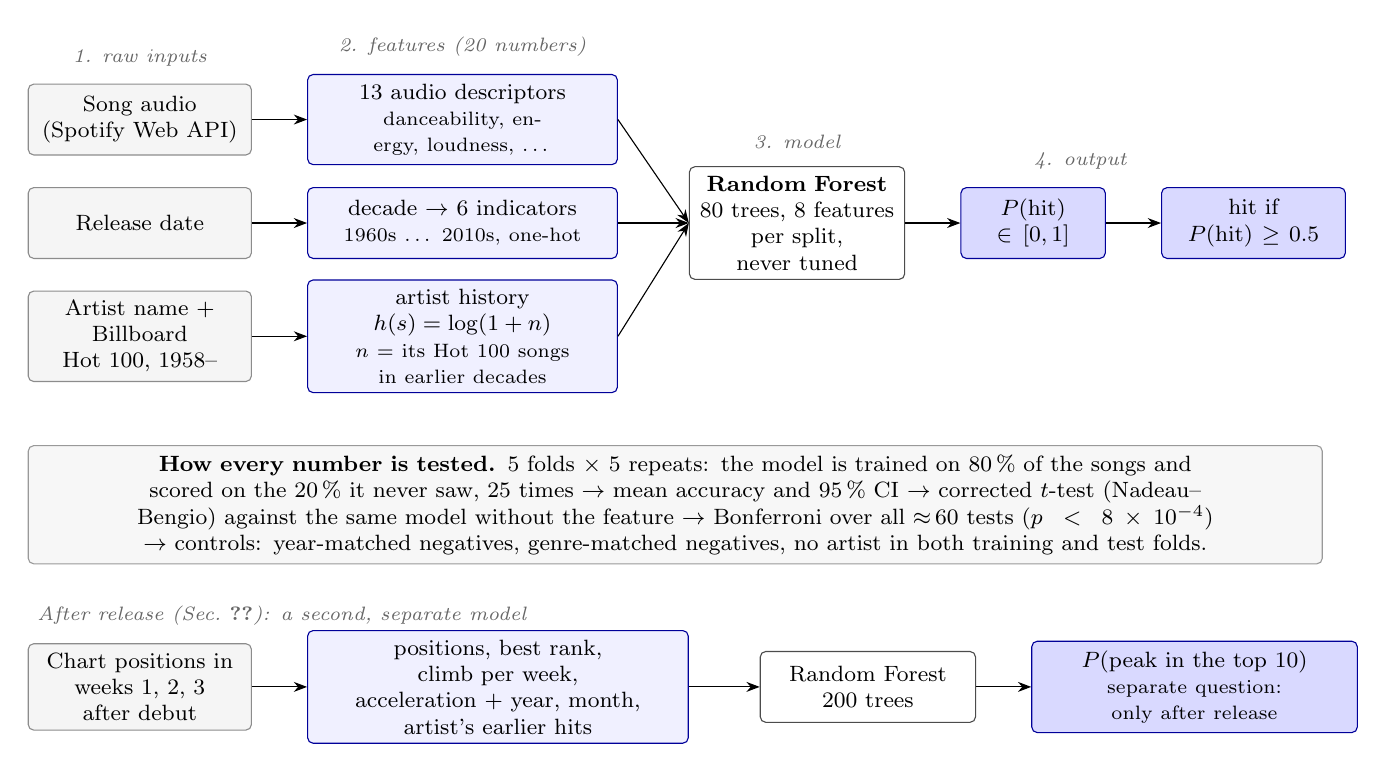
\begin{tikzpicture}[font=\footnotesize, >=Stealth, node distance=4mm,
  src/.style={draw=black!45, fill=black!4, rounded corners=2pt, align=center, text width=2.6cm, minimum height=9mm},
  feat/.style={draw=blue!60!black, fill=blue!6, rounded corners=2pt, align=center, text width=3.7cm, minimum height=9mm},
  stp/.style={draw=black!70, fill=white, rounded corners=2pt, align=center, minimum height=9mm},
  outb/.style={draw=blue!60!black, fill=blue!15, rounded corners=2pt, align=center, minimum height=9mm},
  lab/.style={font=\scriptsize\itshape, text=black!60}]
% ---- inputs
\node[src] (a) {Song audio\\(Spotify Web API)};
\node[src, below=of a] (d) {Release date};
\node[src, below=of d] (h) {Artist name +\\Billboard Hot~100, 1958--};
\node[lab, above=1mm of a] {1. raw inputs};
% ---- features
\node[feat, right=7mm of a] (fa) {13 audio descriptors\\{\scriptsize danceability, energy, loudness, \dots}};
\node[feat, right=7mm of d] (fd) {decade $\rightarrow$ 6 indicators\\{\scriptsize 1960s \dots\ 2010s, one-hot}};
\node[feat, right=7mm of h] (fh) {artist history \mbox{$h(s)=\log(1+n)$}\\{\scriptsize $n$ = its Hot~100 songs in earlier decades}};
\node[lab, above=1mm of fa] {2. features (20 numbers)};
\foreach \x/\y in {a/fa, d/fd, h/fh} \draw[->] (\x) -- (\y);
% ---- model
\node[stp, right=9mm of fd, text width=2.5cm] (rf) {\textbf{Random Forest}\\80 trees, 8 features\\per split, never tuned};
\foreach \x in {fa, fd, fh} \draw[->] (\x.east) -- (rf.west);
\node[lab, above=1mm of rf] {3. model};
\node[outb, right=7mm of rf, text width=1.6cm] (p) {$P(\text{hit})$\\$\in[0,1]$};
\node[outb, right=7mm of p, text width=2.1cm] (dec) {hit if\\$P(\text{hit})\geq 0.5$};
\draw[->] (rf) -- (p);
\draw[->] (p) -- (dec);
\node[lab, above=1mm of p, xshift=6mm] {4. output};
% ---- evaluation band
\node[stp, below=8mm of h.south west, anchor=north west, text width=16.2cm, fill=black!3, draw=black!40] (ev)
 {\textbf{How every number is tested.} 5 folds $\times$ 5 repeats: the model is trained on 80\,\% of the songs and
 scored on the 20\,\% it never saw, 25 times $\rightarrow$ mean accuracy and 95\,\% CI $\rightarrow$ corrected
 $t$-test (Nadeau--Bengio) against the same model without the feature $\rightarrow$ Bonferroni over all
 $\approx$\,60 tests ($p<8\times10^{-4}$) $\rightarrow$ controls: year-matched negatives, genre-matched negatives,
 no artist in both training and test folds.};
% ---- after release
\node[src, below=10mm of ev.south west, anchor=north west, text width=2.6cm] (w) {Chart positions in\\weeks 1, 2, 3 after debut};
\node[feat, right=7mm of w, text width=4.6cm] (wf) {positions, best rank, climb per week,\\acceleration + year, month,\\artist's earlier hits};
\node[stp, right=9mm of wf, text width=2.5cm] (rf2) {Random Forest\\200 trees};
\node[outb, right=7mm of rf2, text width=3.9cm] (p2) {$P(\text{peak in the top 10})$\\\scriptsize separate question: only after release};
\draw[->] (w) -- (wf);
\draw[->] (wf) -- (rf2);
\draw[->] (rf2) -- (p2);
\node[lab, above=1mm of w.north west, anchor=south west] {After release (Sec.~\ref{sec:timeseries}): a second, separate model};
\end{tikzpicture}
\caption{The prediction pipeline. Top: the final model predicts, on release day, whether a song will enter the
Hot~100, from 20 numbers per song. Middle: the protocol under which every gain in this paper is measured. Bottom:
a separate model, used only once a song has charted, predicts whether it will reach the top~10 from its first three
weeks.}
\label{fig:pipeline}
\end{figure*}


\subsection{Overview: what goes in, what comes out}
Fig.~\ref{fig:pipeline} summarises the whole method. The task is binary classification: \emph{input}, one
song described by 20 numbers that are all known on the day it is released (13 audio descriptors, six decade
indicators and the artist's history); \emph{output}, the probability that the song enters the Billboard
Hot~100, turned into a yes/no answer at 0.5. The model is a Random Forest, an ensemble of decision trees that
each ask a sequence of threshold questions about the inputs (``is energy above 0.7?'', ``did the artist
have an earlier hit?'') and then vote. The same pipeline is run on three datasets, each with its own audio
descriptors. Every claimed gain is measured as the difference in held-out accuracy between the pipeline with
and without an input, under the protocol in the middle of the figure. A second, separate pipeline (bottom of the
figure) answers a different question that can only be asked after release.

\subsection{Features}\label{sec:features}
\textbf{Audio.} The 13 Spotify descriptors (Hit Predictor), the 592 Essentia descriptors
(ISMIR) or the 13 Spotify descriptors (SpotGenTrack) form the baseline of each dataset.

\textbf{Era.} On the Hit Predictor we one-hot encode the decade; on ISMIR and SpotGenTrack
we use the decade (or the release year) as a number.

\textbf{Artist history.} Let $a(s)$ be the normalised primary artist of song $s$ (accents,
punctuation and ``feat./\&/with'' collaborators removed) and $t(s)$ its period (decade on
the Hit Predictor, release year elsewhere). With $\mathcal{H}$ the set of reference hits,
\begin{equation}
h(s) = \log\bigl(1 + \bigl|\{\,s' \in \mathcal{H} : a(s') = a(s),\; t(s') < t(s)\,\}\bigr|\bigr).
\end{equation}
The strict inequality guarantees that no information from the song's own period or from
the future is used. In words: for every song, we look up its artist in the full Hot~100
history and count how many different songs that artist had placed on the chart \emph{before}
the song's own decade; the logarithm compresses large counts (an artist with 40 earlier hits is
not twice as likely to chart again as one with 20). Fig.~\ref{fig:history} gives a worked
example. The value is computed separately for every artist and every period, so the same
artist gets a larger value in each later decade, and an artist with no earlier hit always gets
$h(s)=0$.

% Fig.: worked example of the artist-history feature.
\begin{figure}[t]
\centering
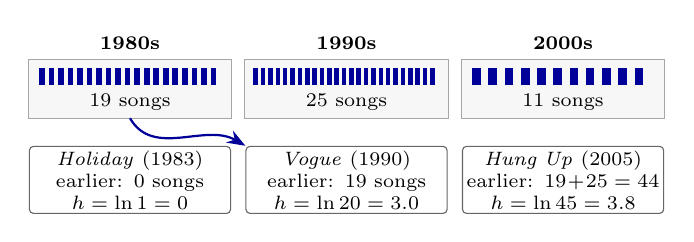
\begin{tikzpicture}[font=\scriptsize, >=Stealth, x=2.75cm, y=1cm,
  ex/.style={draw=black!60, fill=white, rounded corners=1.5pt, align=center, text width=2.45cm, inner sep=1.5pt}]
\foreach \i/\d in {0/1980s, 1/1990s, 2/2000s} {
  \draw[black!35, fill=black!3] (\i,0) rectangle (\i+0.94,0.75);
  \node[anchor=south, font=\scriptsize\bfseries] at (\i+0.47,0.75) {\d};
}
% Madonna's Hot 100 songs, one tick per song
\foreach \k in {0,...,18} \fill[blue!60!black] (0.05+\k*0.044,0.42) rectangle ++(0.026,0.22);
\foreach \k in {0,...,24} \fill[blue!60!black] (1.04+\k*0.034,0.42) rectangle ++(0.021,0.22);
\foreach \k in {0,...,10} \fill[blue!60!black] (2.05+\k*0.075,0.42) rectangle ++(0.04,0.22);
\node at (0.47,0.2) {19 songs};
\node at (1.47,0.2) {25 songs};
\node at (2.47,0.2) {11 songs};
% the three example songs
\node[ex, anchor=north] (s1) at (0.47,-0.35) {\textit{Holiday} (1983)\\earlier: 0 songs\\\mbox{$h=\ln 1=0$}};
\node[ex, anchor=north] (s2) at (1.47,-0.35) {\textit{Vogue} (1990)\\earlier: 19 songs\\\mbox{$h=\ln 20=3.0$}};
\node[ex, anchor=north] (s3) at (2.47,-0.35) {\textit{Hung Up} (2005)\\earlier: $19+25=44$\\\mbox{$h=\ln 45=3.8$}};
\draw[->, blue!60!black, thick] (0.47,0.0) to[out=-60, in=150] (s2.north west);
\end{tikzpicture}
\caption{Artist history, worked example for Madonna. Each tick is one distinct title she had on the Hot~100 in
that decade (decade of the chart week). For a song from the 1990s (\textit{Vogue}), only her songs from
\emph{earlier} decades are counted (the 19 of the 1980s, arrow), never those of the 1990s themselves, so the value
is known on release day. A song from her first hit decade gets 0 (\textit{Holiday}), and a 2000s song counts the
1980s and 1990s ($19+25=44$). $\ln$ is the natural logarithm.}
\label{fig:history}
\end{figure}
 On the Hit Predictor, $\mathcal{H}$ is the full weekly Hot~100 history
(distinct titles per artist and decade); on ISMIR and SpotGenTrack it is the set of positive
songs of the dataset itself. On the Hit Predictor, 52.1\,\% of songs have an artist that
can be matched to the chart history; this includes 99.99\,\% of the hits, and almost all
unmatched songs are flops by artists who never charted (Sec.~\ref{sec:further}).

\textbf{Rich audio.} Standardised and reduced by PCA to 40 components; scaling and PCA are
fitted on the training part of each fold only.

\subsection{Models}
The main model is the Random Forest~\cite{breiman2001random} configuration of Middlebrook
and Sheik~\cite{middlebrook2019song} (80 trees, 8 candidate features per split, Gini),
kept frozen throughout: we do not tune hyperparameters, so that gains come from the
features and remain comparable with the published configuration. Robustness checks use XGBoost~\cite{chen2016xgboost}, logistic
regression, $k$-NN and an RBF support vector machine. External datasets use a Random Forest
with 200 trees and $\sqrt{d}$ candidate features, as in our original external scripts.

\subsection{Evaluation protocol}
We report two estimates for every comparison. The \emph{canonical} estimate reproduces the
split of our earlier experiments (seed 42; 20{,}000 training and 2{,}000 test songs on the
full benchmark, 75/25 elsewhere) and is compared with McNemar's
test~\cite{dietterich1998approximate}. The \emph{cross-validated} estimate uses repeated
stratified 5-fold cross-validation (5 repeats unless stated), reports the mean and a
95\,\% confidence interval, and compares configurations fold by fold with the corrected
resampled $t$-test of Nadeau and Bengio~\cite{nadeau2003inference}. All learned
transformations are inside the cross-validation loop. Title features are produced
out-of-fold: a TF-IDF + logistic-regression model is trained within the training part and
its predicted probability is used as a single feature.

\textbf{Two kinds of ``new'' artist.} Two different situations are easy to confuse, and we keep
them apart throughout. An \emph{unseen} artist is one whose songs are absent from the training
folds; its chart history before the song is still known, so $h(s)$ can be positive. We test unseen
artists with artist-grouped cross-validation (Sec.~\ref{sec:robust}), to check that the model does
not simply recognise artists it was trained on. A \emph{new} (cold-start) artist is one with no
earlier Hot~100 song, so $h(s)=0$ by definition, and artist history cannot help them. Our claims
that the gain ``holds for unseen artists'' never mean that it helps new artists; for new artists
only era and audio are informative (Table~\ref{tab:robust}).

\subsection{How inputs were selected}\label{sec:selection}
% Fig.: how a candidate input is kept or rejected.
\begin{figure}[t]
\centering
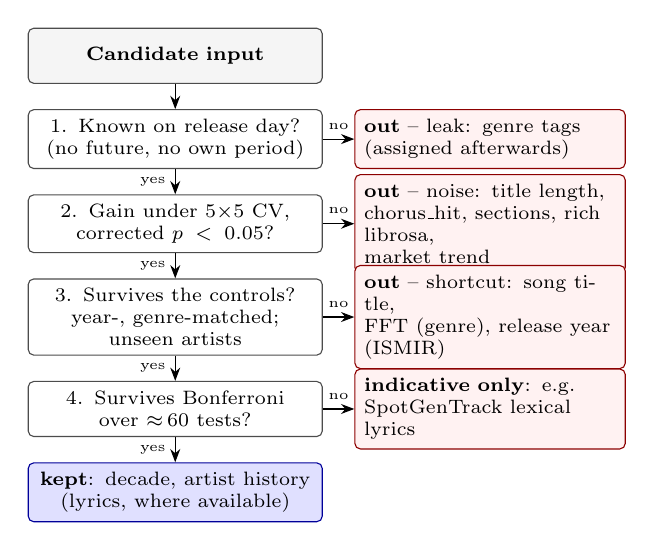
\begin{tikzpicture}[font=\scriptsize, >=Stealth, node distance=3.2mm,
  q/.style={draw=black!70, fill=white, rounded corners=2pt, align=center, text width=3.5cm, minimum height=7mm},
  no/.style={draw=red!55!black, fill=red!5, rounded corners=2pt, align=left, text width=3.2cm, minimum height=7mm},
  yes/.style={draw=blue!60!black, fill=blue!12, rounded corners=2pt, align=center, text width=3.5cm, minimum height=7mm}]
\node[q, fill=black!4] (c) {\textbf{Candidate input}};
\node[q, below=of c] (q1) {1. Known on release day?\\(no future, no own period)};
\node[q, below=of q1] (q2) {2. Gain under $5{\times}5$ CV,\\corrected $p<0.05$?};
\node[q, below=of q2] (q3) {3. Survives the controls?\\year-, genre-matched; unseen artists};
\node[q, below=of q3] (q4) {4. Survives Bonferroni\\over $\approx$\,60 tests?};
\node[yes, below=of q4] (k) {\textbf{kept}: decade, artist history\\(lyrics, where available)};
\node[no, right=4mm of q1] (n1) {\textbf{out} -- leak: genre tags\\(assigned afterwards)};
\node[no, right=4mm of q2] (n2) {\textbf{out} -- noise: title length,\\chorus\_hit, sections, rich librosa,\\market trend};
\node[no, right=4mm of q3] (n3) {\textbf{out} -- shortcut: song title,\\FFT (genre), release year (ISMIR)};
\node[no, right=4mm of q4] (n4) {\textbf{indicative only}: e.g.\\SpotGenTrack lexical lyrics};
\draw[->] (c) -- (q1);
\foreach \a/\b in {q1/q2, q2/q3, q3/q4, q4/k} \draw[->] (\a) -- node[left, font=\tiny] {yes} (\b);
\foreach \a/\b in {q1/n1, q2/n2, q3/n3, q4/n4} \draw[->] (\a) -- node[above, font=\tiny] {no} (\b);
\end{tikzpicture}
\caption{How every candidate input was kept or rejected. Each input is tested in this order; the boxes on the right
list the inputs that stopped at each question.}
\label{fig:selection}
\end{figure}

We did not choose the inputs in advance. Every candidate we built---decade, artist history, song title,
title length, \texttt{chorus\_hit}/\texttt{sections}, a 185-dimensional librosa representation, 31 FFT
descriptors, Spotify artist genres, market-trend features and lyrics---went through the same four
questions (Fig.~\ref{fig:selection}). We first ask whether the input is known on release day. We then
measure its gain under $5{\times}5$ cross-validation with the corrected $t$-test, not on one split. We
then re-test it under the controls that remove the known construction shortcuts of each dataset: negatives
matched by year (ISMIR), negatives matched by genre (Hit Predictor), and no artist shared between training
and test folds. Finally we require significance after a Bonferroni correction over all the tests in the
paper. We call an input that passes all four questions a \emph{surviving} input, and we rank all tested gains
by this criterion in Table~\ref{tab:survival} (the \emph{survival ranking}). Only two inputs survive on every
dataset: decade (which matters only through its interactions with audio) and artist history. Lyrics survive on
the one dataset where we could attach them to both hits and non-hits (Sec.~\ref{sec:lyrics}). We also trained
a model on everything at once, and we removed one input at a time from both that model and the final model
(Sec.~\ref{sec:ablation}).

% =====================================================================
\section{Results}

\subsection{Main result on the Spotify Hit Predictor}\label{sec:main}

\begin{table}[t]
\centering
\caption{Spotify Hit Predictor (40{,}560 songs), frozen Random Forest. Canonical split
(2{,}000 test songs, McNemar) and $5{\times}5$ cross-validation (mean, 95\,\% CI, corrected
$t$-test, folds improved out of 25).}
\label{tab:main}
\footnotesize
\setlength{\tabcolsep}{2.4pt}
\begin{adjustbox}{max width=\columnwidth}
\begin{tabular}{@{}lccccc@{}}
\toprule
& \multicolumn{2}{c}{Canonical} & \multicolumn{3}{c}{Cross-validation} \\
\cmidrule(lr){2-3}\cmidrule(l){4-6}
Features & Acc. & $p$ & Acc. [95\,\% CI] & AUC & $p$ (wins) \\
\midrule
Audio (13) & .773 & -- & .782 [.780,.784] & .859 & -- \\
+ decade & .796 & $3{\cdot}10^{-4}$ & .802 [.800,.804] & .880 & $10^{-10}$ (25) \\
+ artist & .800 & $6{\cdot}10^{-4}$ & .810 [.808,.813] & .900 & $10^{-11}$ (25) \\
\textbf{+ decade + artist} & \textbf{.822} & $2{\cdot}10^{-9}$ & \textbf{.832 [.830,.834]} & \textbf{.918} & $7{\cdot}10^{-17}$ (25) \\
Decade + artist only & .668 & -- & .670 [.669,.672] & .685 & -- \\
\bottomrule
\end{tabular}
\end{adjustbox}
\end{table}

\begin{figure}[t]
\centering
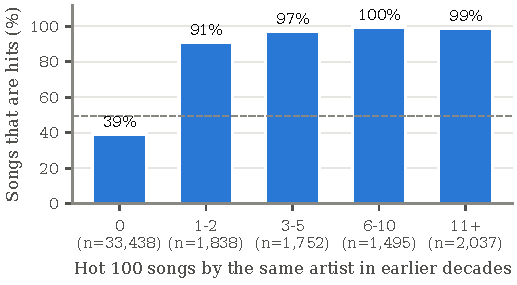
\includegraphics[width=\columnwidth]{fig_artist_curve.pdf}
\caption{Share of hits by the number of Hot~100 songs the artist placed in earlier decades
(Spotify Hit Predictor, 40{,}560 songs). Dashed line: overall hit share (49\,\%).}
\label{fig:artist}
\end{figure}

Table~\ref{tab:main} shows that each feature helps on its own and that their gains are
nearly additive. The canonical numbers reproduce our earlier single-split experiments
exactly; cross-validation places all accuracies about one point higher and gives very
narrow intervals. The combined gain is $+5.04$\pp{} and is positive in all 25 folds.
It is not bought by trading recall for precision: on the hit class, precision rises from
0.758 to 0.828 and recall from 0.819 to 0.833, so F1 rises from 0.787 to 0.831 ($+4.3$\pp,
25/25, $p=7\times10^{-15}$).
Without audio the two features reach only 0.670, so they complement rather than replace
the descriptors. The relation between artist history and the label is strongly nonlinear
(Fig.~\ref{fig:artist}):
39.3\,\% of the 33{,}438 songs whose artist had no earlier hit are hits, against 91.0\,\%
for one or two earlier hits and 97.2--99.6\,\% beyond.

\begin{table}[t]
\centering
\caption{Cross-validated accuracy per decade (Random Forest).}
\label{tab:decade}
\footnotesize
\setlength{\tabcolsep}{3.2pt}
\begin{adjustbox}{max width=\columnwidth}
\begin{tabular}{@{}lcccccc@{}}
\toprule
Features & 60s & 70s & 80s & 90s & 00s & 10s \\
\midrule
Audio (13) & .743 & .750 & .770 & .806 & .836 & .816 \\
+ decade & .764 & .763 & .794 & .840 & .851 & .833 \\
+ artist & .763 & .784 & .812 & .831 & .860 & .842 \\
+ decade + artist & \textbf{.788} & \textbf{.796} & \textbf{.836} & \textbf{.864} & \textbf{.873} & \textbf{.868} \\
\bottomrule
\end{tabular}
\end{adjustbox}
\end{table}

The improvement holds in every decade (Table~\ref{tab:decade}), from $+3.7$\pp{} in the
2000s to $+6.6$\pp{} in the 1980s. Since each decade file is balanced, the decade indicator
carries no information on its own; its gain can only come from interactions with the audio
descriptors, i.e.\ from era-specific decision rules.

\begin{table}[t]
\centering
\caption{Robustness to the classifier (5-fold CV, corrected $t$-test; all 5 folds improve).}
\label{tab:models}
\footnotesize
\setlength{\tabcolsep}{3pt}
\begin{adjustbox}{max width=\columnwidth}
\begin{tabular}{@{}lcccc@{}}
\toprule
Classifier & Audio (13) & + decade + artist & $\Delta$ & $p$ \\
\midrule
Random Forest~\cite{breiman2001random} & .780 & .832 & +5.2 & $2{\cdot}10^{-5}$ \\
XGBoost~\cite{chen2016xgboost} & .788 & \textbf{.845} & +5.7 & $3{\cdot}10^{-7}$ \\
Logistic regression & .727 & .782 & +5.5 & $4{\cdot}10^{-5}$ \\
$k$-NN ($k=25$) & .750 & .796 & +4.6 & $8{\cdot}10^{-6}$ \\
SVM (RBF) & .773 & .828 & +5.5 & $3{\cdot}10^{-5}$ \\
\bottomrule
\end{tabular}
\end{adjustbox}
\end{table}

\textbf{Robustness to the classifier.} The gain is of the same size for five classifiers of
very different nature (Table~\ref{tab:models}), so it comes from the features rather than
from the model. XGBoost is the strongest on average, but on the canonical split it ties with
the frozen Random Forest (0.820 vs 0.822, McNemar $p=0.87$). TreeSHAP attributions of the
XGBoost model rank artist history first (mean $|\phi|=1.08$), the six decade indicators
second (0.86 summed) and instrumentalness third (0.73), ahead of every other descriptor.

\textbf{Future decades.} To test whether the gain survives a temporal shift, we train on all
earlier decades and test on a later one, with no song from the test decade seen in
training. Artist history improves the Random Forest by $+2.5$\pp{} on the 1990s
(0.736 $\to$ 0.761), $+1.9$\pp{} on the 2000s (0.805 $\to$ 0.824) and $+3.4$\pp{} on the
2010s (0.780 $\to$ 0.814; McNemar $p$ between $10^{-7}$ and $10^{-21}$), with similar gains
for XGBoost. The decade indicator cannot be used here, since the test decade never
appears in training.

\subsection{Where the accuracy comes from}\label{sec:ablation}

\textbf{Which descriptors matter: PCA.} To see which of the 13 Spotify descriptors carry the
signal, we ran a principal component analysis on the standardised descriptors
(Fig.~\ref{fig:pca}). The first component (23.6\,\% of the variance) is an \emph{intensity} axis
(energy $+0.48$, loudness $+0.47$, acousticness $-0.43$) and is also the one that best separates hits
(ROC-AUC 0.70 on its own). The second (11.1\,\%) is a \emph{mood} axis (danceability $+0.48$,
valence $+0.44$, duration $-0.36$; AUC 0.62). The next four components together explain another
33\,\% of the variance but separate hits no better than chance (AUC 0.50--0.52), and eight components
are needed to reach 81\,\%. Variance and usefulness therefore do not coincide. Among single descriptors,
the most separating are instrumentalness (AUC 0.74, lower in hits), danceability (0.70, higher),
loudness (0.64) and valence (0.64); key, duration and tempo are close to chance (0.51--0.52). Replacing
the descriptors by their components only loses accuracy: the frozen Random Forest reaches 0.575 with
one component, 0.710 with six and 0.765 with all 13, against 0.782 for the raw descriptors ($-1.7$\pp{}
even though no information is removed, 0/25 folds, $p=2\times10^{-8}$). Trees split on one input at a
time, and rotating the axes mixes a sparse, highly informative descriptor (instrumentalness) into
components shared with uninformative ones. We therefore keep the raw descriptors; PCA is used only for the
185-dimensional librosa representation (Sec.~\ref{sec:audit}).

\begin{figure*}[t]
\centering
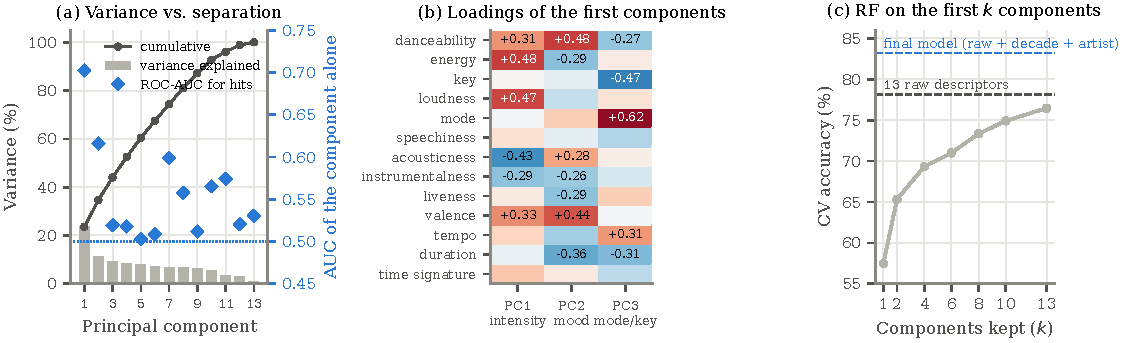
\includegraphics[width=\textwidth]{fig_pca.pdf}
\caption{PCA of the 13 Spotify descriptors (40{,}560 songs). (a) Variance explained by each component
(bars), cumulative (line), and how well each component alone separates hits from non-hits (ROC-AUC, right
axis; dotted line = chance). (b) Loadings of the first three components (values below 0.25 in absolute
value are not printed). (c) Cross-validated accuracy of the frozen Random Forest trained on the first $k$
components, against the 13 raw descriptors and the final model.}
\label{fig:pca}
\end{figure*}

\textbf{Ablation: remove one input at a time.} To see where the power of the final model comes from, we
removed each of its inputs in turn and re-ran the $5{\times}5$ cross-validation, comparing every reduced
model with the full one fold by fold (Fig.~\ref{fig:ablation}a). Removing artist history costs the most
($-3.0$\pp, 0/25 folds better, $p=7\times10^{-13}$), then the decade indicators ($-2.2$\pp,
$p=5\times10^{-13}$), instrumentalness ($-1.6$\pp, $p=6\times10^{-9}$) and duration ($-1.1$\pp,
$p=2\times10^{-7}$). These four survive the Bonferroni correction. Acousticness, speechiness, energy,
danceability and valence each cost 0.3--0.6\pp{} ($0.004\leq p\leq0.04$), because the other descriptors
largely carry the same information. Removing key, liveness, time signature, mode or tempo changes nothing
($p\geq0.30$). Keeping one block alone shows that the blocks are complementary rather than redundant: the
13 descriptors alone reach 0.782, artist history alone 0.670, the decade alone 0.503 (chance, since every
decade is balanced), and all three together 0.832. Removing all 13 descriptors at once costs $-16.2$\pp.
So audio carries most of the accuracy, and artist history and era add to it.

\textbf{Permutation importance.} Removing an input lets the model re-learn with the others, so
correlated descriptors can stand in for one another. As a second view, we shuffle one input at a time in the
held-out folds of the trained final model, which measures how much the model relies on it
(Fig.~\ref{fig:ablation}b). The ranking is the same at the top: artist history (8.9\pp{} lost when shuffled),
then instrumentalness (6.3), acousticness (4.9), the decade block (4.3), duration (3.9) and danceability
(3.4), with key, liveness and time signature near zero. Duration is an instructive case. On its own it barely
separates hits (AUC 0.51; Appendix~\ref{app:inputs}), but the model relies on it, presumably because song lengths
changed across decades and its effect depends on the era. Its value comes from interactions, like that of the
decade.

\begin{figure*}[t]
\centering
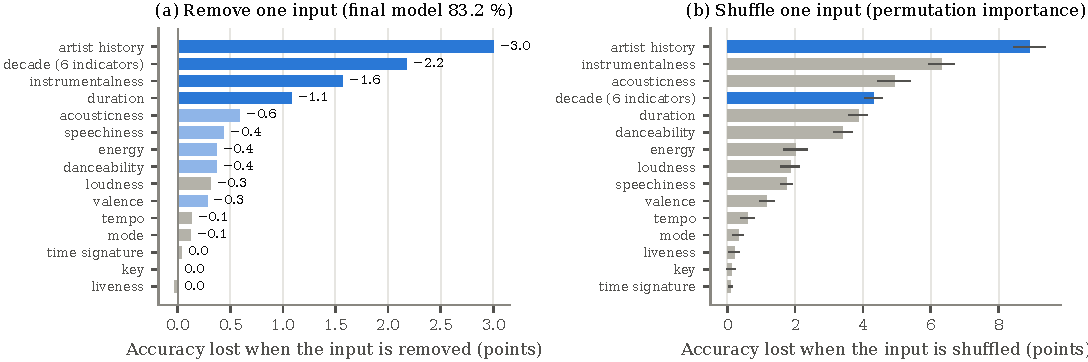
\includegraphics[width=\textwidth]{fig_ablation.pdf}
\caption{Where the accuracy of the final model comes from (Hit Predictor, 40{,}560 songs). (a) Accuracy lost
when one input is removed and the model is retrained ($5{\times}5$ CV; dark blue: significant after Bonferroni,
light blue: $p<0.05$, gray: not significant). (b) Accuracy lost when one input is shuffled in the held-out
folds of the trained model (5 folds $\times$ 5 shuffles, mean $\pm$ s.d.). Blue: non-audio inputs.}
\label{fig:ablation}
\end{figure*}

\textbf{Training on everything at once.} One might simply put every input we built into one model. We did
this on the 35{,}370 songs that have a preview (needed for FFT), with the same frozen Random Forest and
$5{\times}5$ CV (Table~\ref{tab:all}). The full model reaches 0.883, 5.8 points above the final model
(0.825 on these songs). That gain does not come from music. Removing the song title alone takes it down to
0.843 ($-4.0$\pp, $p=3\times10^{-19}$), and the title is an artefact of how the non-hits were collected
(Sec.~\ref{sec:audit}). The remaining $+1.8$\pp{} over the final model comes from FFT and the market-trend
features (removing them costs $-0.4$ and $-0.3$\pp), whose gains vanish under the genre control and carry
only the era (Sec.~\ref{sec:further}, \ref{sec:timeseries}). Once FFT and trend are in, the decade
indicators become redundant ($-0.2$\pp, $p=0.11$): all three describe the era. Artist history remains the
input whose removal costs the most among the legitimate ones ($-1.9$\pp, $p=2\times10^{-11}$), ahead of
the 13 descriptors ($-1.2$\pp), while \texttt{chorus\_hit}/\texttt{sections} and title length change nothing.
Training on everything therefore gives a higher number on this benchmark by learning how it was built. The
model we keep is the one whose inputs survive the controls: the 20 inputs of the final model.

\begin{table}[t]
\centering
\caption{Training on every input at once (35{,}370 songs with a preview, frozen Random Forest, $5{\times}5$
CV). Left: one block removed from ``everything'' ($\Delta$ vs everything). Right: the block alone.}
\label{tab:all}
\footnotesize
\setlength{\tabcolsep}{3pt}
\begin{adjustbox}{max width=\columnwidth}
\begin{tabular}{@{}lccc@{}}
\toprule
Model & Acc. & AUC & $\Delta$ ($p$) \\
\midrule
Final model (Spotify + decade + artist) & .825 & .911 & -- \\
Everything (8 blocks) & \textbf{.883} & .952 & +5.8 ($3{\cdot}10^{-21}$) vs final \\
Everything except song title & .843 & .925 & +1.8 ($6{\cdot}10^{-10}$) vs final \\
\midrule
\multicolumn{4}{@{}l}{\emph{Remove one block from everything}} \\
\quad $-$ song title & .843 & .925 & $-4.0$ ($3{\cdot}10^{-19}$) \\
\quad $-$ artist history & .864 & .933 & $-1.9$ ($2{\cdot}10^{-11}$) \\
\quad $-$ Spotify (13) & .871 & .944 & $-1.2$ ($5{\cdot}10^{-8}$) \\
\quad $-$ FFT (31) & .879 & .949 & $-0.4$ (.01) \\
\quad $-$ market trend (2) & .879 & .949 & $-0.3$ (.01) \\
\quad $-$ decade (6) & .881 & .950 & $-0.2$ (.11) \\
\quad $-$ title length & .883 & .951 & $-0.0$ (.93) \\
\quad $-$ chorus\_hit + sections & .883 & .952 & $+0.0$ (.75) \\
\midrule
\multicolumn{4}{@{}l}{\emph{One block alone}} \\
\quad Spotify (13) / FFT (31) & .777 / .773 & .849 / .847 & -- \\
\quad artist history / song title & .648 / .660 & .669 / .740 & -- \\
\quad market trend / title length & .629 / .546 & .672 / .545 & -- \\
\quad chorus\_hit + sections / decade & .543 / .532 & .563 / .516 & -- \\
\bottomrule
\end{tabular}
\end{adjustbox}
\end{table}

\subsection{Head-to-head with prior work on the same benchmark}\label{sec:tilburg}

\begin{table}[t]
\centering
\caption{Head-to-head with Du~\cite{du2022spotify} using their protocol (one model per
decade, 13 audio + \texttt{chorus\_hit} + \texttt{sections}, 70/30 split) over 50 random
splits: mean accuracy (std). ``Wins'' counts splits where adding artist history helps.}
\label{tab:tilburg}
\footnotesize
\setlength{\tabcolsep}{2.6pt}
\begin{adjustbox}{max width=\columnwidth}
\begin{tabular}{@{}llcccc@{}}
\toprule
Dec. & Model & Published & Re-impl. & + artist & Wins / $p$ \\
\midrule
\multirow{3}{*}{00s} & RF (their cfg.) & .84 & .846 (.009) & \textbf{.867} (.009) & 50 / $9{\cdot}10^{-8}$ \\
& LR (their cfg.) & .82 & .821 (.007) & \textbf{.848} (.007) & 50 / $2{\cdot}10^{-9}$ \\
& RF (frozen) & -- & .852 (.008) & \textbf{.875} (.006) & 50 / $10^{-7}$ \\
\midrule
\multirow{3}{*}{10s} & RF (their cfg.) & .82 & .829 (.008) & \textbf{.861} (.008) & 50 / $4{\cdot}10^{-11}$ \\
& LR (their cfg.) & .79 & .807 (.009) & \textbf{.835} (.008) & 50 / $6{\cdot}10^{-6}$ \\
& RF (frozen) & -- & .841 (.008) & \textbf{.873} (.008) & 50 / $9{\cdot}10^{-10}$ \\
\bottomrule
\end{tabular}
\end{adjustbox}
\end{table}

\begin{figure}[t]
\centering
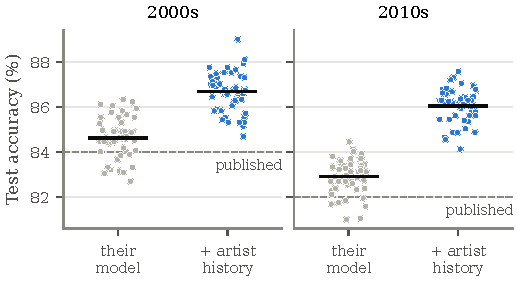
\includegraphics[width=\columnwidth]{fig_tilburg.pdf}
\caption{Head-to-head with Du~\cite{du2022spotify}: accuracy of their Random Forest over 50
random 70/30 splits (dots; bar = mean), without (gray) and with (blue) artist history.
Dashed line: their published accuracy.}
\label{fig:tilburg}
\end{figure}

Du~\cite{du2022spotify} trained one Random Forest (450 trees, $m_{\text{try}}=2$, at most
30 leaves) and one logistic regression per decade on the 2000s and 2010s, with a single
70/30 split. Because the original R random seed cannot be replayed, we repeat the split
with 50 seeds. Our re-implementation lands on or slightly above the published figures
(Table~\ref{tab:tilburg}, Fig.~\ref{fig:tilburg}), which validates the protocol. Adding artist history to
\emph{their} models, with \emph{their} inputs, improves accuracy by $+2.1$ to $+3.2$\pp{}
on every split, and the improved models exceed the published accuracy on 100\,\% of the
splits. The decade feature is constant within a per-decade model and is therefore not used
here.

\subsection{External validation}\label{sec:external}

\begin{table}[t]
\centering
\caption{ISMIR 2019 data, Random Forest on 592 Essentia descriptors, $5{\times}2$
cross-validation. A: balanced random negatives (as in~\cite{zangerle2019hit}). B: negatives
matched to hits year by year. $p$: corrected $t$-test vs audio; all 10 folds improve where
significant.}
\label{tab:ismir}
\footnotesize
\setlength{\tabcolsep}{2.8pt}
\begin{adjustbox}{max width=\columnwidth}
\begin{tabular}{@{}lcccc@{}}
\toprule
& \multicolumn{2}{c}{A: random negatives} & \multicolumn{2}{c}{B: year-matched} \\
\cmidrule(lr){2-3}\cmidrule(l){4-5}
Features & Acc. [95\,\% CI] & $p$ & Acc. [95\,\% CI] & $p$ \\
\midrule
Audio (Essentia) & .708 [.700,.717] & -- & .682 [.677,.688] & -- \\
+ year & .739 [.734,.744] & $2{\cdot}10^{-4}$ & .681 [.674,.688] & .66 \\
+ artist & .733 [.727,.740] & $2{\cdot}10^{-5}$ & \textbf{.708} [.702,.714] & $3{\cdot}10^{-5}$ \\
\textbf{+ year + artist} & \textbf{.763} [.758,.768] & $7{\cdot}10^{-8}$ & \textbf{.708} [.702,.715] & $3{\cdot}10^{-5}$ \\
Year alone & .702 [.697,.707] & -- & .448 [.444,.451] & -- \\
\midrule
\multicolumn{5}{@{}l}{Best published~\cite{zangerle2019hit}: 75.04\,\% (wide-and-deep, audio + year, 5-fold CV)} \\
\bottomrule
\end{tabular}
\end{adjustbox}
\end{table}

\textbf{ISMIR 2019.} (Table~\ref{tab:ismir}, Fig.~\ref{fig:ismir}.) With random balanced negatives (protocol A, as in the original
study), release year alone reaches 70.2\,\%---as much as 592 audio descriptors---because
hits and non-hits come from different eras. Audio + year, which mirrors the inputs of the
best model of Zangerle et~al., reaches 73.9\,\%; adding artist history raises it to
76.3\,\% ($+2.4$\pp, 10/10 folds, $p=7\times10^{-8}$), above the published 75.04\,\%.
Protocol B removes the era shortcut by drawing, for every hit, a non-hit from the same
release year. Year and decade then become useless ($p>0.5$, and year alone falls below
chance), while artist history still adds $+2.6$\pp{} ($p=3\times10^{-5}$, 10/10 folds).
This is the cleanest estimate of the feature's value: the negatives are not selected by
artist and cannot be separated by date.

\begin{figure}[t]
\centering
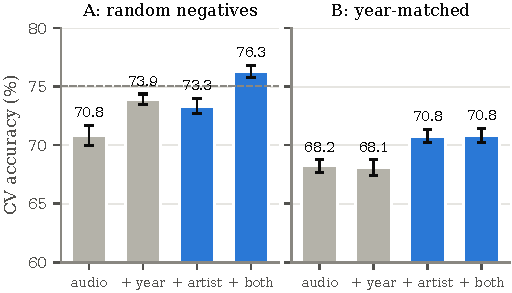
\includegraphics[width=\columnwidth]{fig_ismir.pdf}
\caption{ISMIR 2019 data, cross-validated accuracy with 95\,\% CI. Gray: without artist
history; blue: with it (``both'' = year + artist). Dashed line in A: best published
accuracy~\cite{zangerle2019hit}. Matching years (B) removes the gain of release year but not
that of artist history.}
\label{fig:ismir}
\end{figure}

\begin{table}[t]
\centering
\caption{SpotGenTrack (101{,}909 tracks, 19.4\,\% hits; always predicting ``non-hit''
scores 0.806). 5-fold CV, corrected $t$-test vs the 13 descriptors.}
\label{tab:sgt}
\footnotesize
\setlength{\tabcolsep}{3pt}
\begin{adjustbox}{max width=\columnwidth}
\begin{tabular}{@{}lccc@{}}
\toprule
Features & Acc. [95\,\% CI] & ROC-AUC & $p$ (acc.) \\
\midrule
Spotify descriptors (13) & .812 [.811,.813] & .690 & -- \\
+ decade & .812 [.811,.813] & .712 & .66 \\
+ artist & .823 [.821,.826] & .762 & $10^{-3}$ \\
\textbf{+ decade + artist} & \textbf{.825} [.823,.827] & \textbf{.777} & $3{\cdot}10^{-4}$ \\
+ artist + low-level audio & .825 [.823,.828] & .758 & $2{\cdot}10^{-4}$ \\
\bottomrule
\end{tabular}
\end{adjustbox}
\end{table}

\textbf{SpotGenTrack.} Here the label is Spotify popularity rather than a chart, and
80.6\,\% of tracks are negatives, so accuracy is dominated by the majority class: the 13
descriptors score 0.812, barely above always predicting ``non-hit''. Ranking quality tells
the real story (Table~\ref{tab:sgt}): artist history raises ROC-AUC from 0.690 to 0.762
($+7.2$ points), and with decade to 0.777. On the hit class, the 13 descriptors find
only 8.3\,\% of the hits (F1 0.147); with decade and artist history, recall rises to
25.2\,\% at unchanged precision (0.62) and F1 to 0.358 (5/5 folds, $p=7\times10^{-7}$),
while the 207 low-level audio features add
nothing on top of artist history. A single 75/25 split gives the same picture (accuracy
0.810 $\to$ 0.822 and ROC-AUC 0.688 $\to$ 0.760 with artist history, McNemar
$p=6\times10^{-13}$).

\subsection{Unseen artists and cold start}\label{sec:robust}

\begin{table}[t]
\centering
\caption{Robustness. Top: cross-validated accuracy with random stratified folds vs folds
grouped by artist (no test artist seen in training). Era = decade (Hit Predictor) or
release year (ISMIR). Bottom: gain over audio in grouped CV, on songs whose artist had no
earlier hit (new) or at least one (known). New/known songs: 33{,}438/7{,}122 (Hit
Predictor), 7{,}480/4{,}182 (ISMIR A), 7{,}269/4{,}393 (ISMIR B).}
\label{tab:robust}
\footnotesize
\setlength{\tabcolsep}{2.6pt}
\begin{adjustbox}{max width=\columnwidth}
\begin{tabular}{@{}llcccc@{}}
\toprule
Data & Folds & Audio & + era & + artist & + both \\
\midrule
\multirow{2}{*}{Hit Predictor} & random & .782 & .802 & .810 & .832 \\
 & by artist & .772 & .792 & .802 & \textbf{.822} \\
\multirow{2}{*}{ISMIR A} & random & .708 & .739 & .733 & .763 \\
 & by artist & .709 & .739 & .730 & \textbf{.759} \\
\multirow{2}{*}{ISMIR B} & random & .682 & .681 & .708 & .708 \\
 & by artist & .677 & .678 & \textbf{.705} & \textbf{.705} \\
\midrule
& Hits (\%) & \multicolumn{2}{c}{New artists: $\Delta$ ($p$)} & \multicolumn{2}{c}{Known: $\Delta$ ($p$)} \\
\cmidrule(lr){3-4}\cmidrule(l){5-6}
& new/known & + era & + artist & \multicolumn{2}{c}{+ artist} \\
\midrule
Hit Predictor & 39 / 97 & +2.2 ($2{\cdot}10^{-9}$) & +0.4 (.17) & \multicolumn{2}{c}{+15.0 ($3{\cdot}10^{-14}$)} \\
ISMIR A & 36 / 75 & +3.4 ($6{\cdot}10^{-5}$) & +0.8 (.08) & \multicolumn{2}{c}{+4.4 (.003)} \\
ISMIR B & 37 / 72 & +0.1 (.79) & +1.4 (.002) & \multicolumn{2}{c}{+5.3 ($8{\cdot}10^{-5}$)} \\
\bottomrule
\end{tabular}
\end{adjustbox}
\end{table}

\textbf{Artist-grouped cross-validation.} With random folds, songs by the same artist can
fall in both the training and the test part, so a model could recognise an artist from the
audio. We therefore repeat every protocol with stratified group $k$-fold, grouping songs by
normalised artist so that no test artist is seen in training (Table~\ref{tab:robust}, top).
Accuracies drop by up to one point, a small artist-identity effect in the audio
descriptors, but the gains remain: $+5.0$\pp{} for decade and artist on the Hit
Predictor (unchanged, 25/25 folds, $p=10^{-13}$) and $+2.9$\pp{} for artist history in the
year-matched ISMIR protocol (10/10, $p=9\times10^{-7}$). In protocol A the gains lose at
most half a point, and audio, year and artist still reach 0.759 [0.752, 0.766], above the
published 75.04\,\%.

\textbf{Cold start.} Table~\ref{tab:robust} (bottom) splits the grouped test folds by
whether the artist had an earlier hit. On the Hit Predictor, artist history does not help
new artists ($+0.4$\pp, $p=0.17$): its whole gain comes from the 17.6\,\% of songs by
established artists, 96.6\,\% of which are hits, which quantifies the benchmark effect
discussed in Sec.~\ref{sec:discussion}. The decade, in contrast, helps new artists
($+2.2$\pp, $p=2\times10^{-9}$). On ISMIR, where songs by established artists are hits
only 72--75\,\% of the time, artist history also tends to help new artists in the year-matched
protocol ($+1.4$\pp, $p=0.002$, 10/10 folds), presumably because an empty chart history is itself
informative when negatives are not selected by artist.

\subsection{Audit: which gains are not real}\label{sec:audit}

\begin{table}[t]
\centering
\caption{Audit of candidate gains. Single split (McNemar) vs $5{\times}5$ cross-validation
(corrected $t$-test). Top: full benchmark. Bottom: 3{,}562-song audio subset.}
\label{tab:audit}
\footnotesize
\setlength{\tabcolsep}{2.6pt}
\begin{adjustbox}{max width=\columnwidth}
\begin{tabular}{@{}lcccl@{}}
\toprule
Added to audio & Split $\Delta$ ($p$) & CV $\Delta$ & CV $p$ & Verdict \\
\midrule
Song title (TF-IDF) & +6.9 ($4{\cdot}10^{-14}$) & +6.7 & $4{\cdot}10^{-20}$ & artefact \\
\texttt{chorus\_hit}+\texttt{sections} & +0.6 (.32) & $-$0.0 & .82 & no effect \\
Title length & +0.05 (1.0) & +0.2 & .28 & no effect \\
\midrule
Rich librosa (PCA 40) & +3.8 (.002) & +0.9 & .15 & not significant \\
FFT descriptors (31) & +4.4 (.001) & +2.3 & .007 & small \\
Decade & +1.1 (.27) & +1.0 & .03 & small \\
Artist & +3.4 (.010) & +3.8 & $2{\cdot}10^{-6}$ & robust \\
Artist + rich & +6.7 ($10^{-6}$) & +4.9 & $10^{-8}$ & = artist \\
Decade + artist & +3.6 (.006) & +5.1 & $10^{-8}$ & robust \\
\bottomrule
\end{tabular}
\end{adjustbox}
\end{table}

\textbf{Titles.} A title model trained out-of-fold adds $+6.7$\pp, more than any musical
feature. Titles do not make songs popular; they reveal the construction of the benchmark,
whose non-hits are drawn from niche genres and catalogue releases whose titles differ
systematically from Hot~100 singles. We reject this feature despite its significance.

\textbf{Single split vs cross-validation.} On the small audio subset, the 185 rich librosa
descriptors appeared to add $+3.8$\pp{} with $p=0.002$ on the canonical split, but the
cross-validated gain is $+0.9$\pp{} and is not significant. The same holds for the choice
of the PCA dimension (5 to 100 components are within noise) and for the knock-out of any
descriptor family (all within $\pm0.1$\pp). In a block ablation of the full subset model,
only removing artist history causes a significant drop ($-3.3$\pp, $p=10^{-5}$). The
\texttt{chorus\_hit} and \texttt{sections} fields, often suspected of leakage, add nothing.

\textbf{FFT and the best audio-subset model.} The 31 FFT descriptors are the only extra
audio representation whose gain survives cross-validation, and it persists on top of
artist history: audio + artist + FFT reaches $0.821$ against $0.801$ for audio + artist
($+2.0$\pp, 23/25 folds, $p=0.008$). Adding decade to that model gives the best subset
accuracy, $0.824$, but the increment is not significant ($+0.3$\pp, $p=0.50$), and
decade adds nothing to FFT alone ($0.786$ vs $0.785$): the spectral descriptors already
carry the era. Conversely, artist history still adds $+3.5$\pp{} on top of FFT
($p=4\times10^{-5}$). Fig.~\ref{fig:subset} shows every configuration we evaluated on
this subset.

\textbf{FFT on the whole benchmark.} We then retrieved Deezer previews for every song we
could match: 35{,}370 of the 40{,}560 songs (87.2\,\%). Deezer finds hits more often than
flops (94.0\,\% vs 80.6\,\%), so the covered set is 53.2\,\% hits and every comparison
below uses the same 35{,}370 songs. With $5{\times}5$ cross-validation, adding FFT to the
main model (audio + decade + artist) raises accuracy from $0.825$ to $0.839$ ($+1.4$\pp,
25/25 folds, $p=4\times10^{-9}$; AUC $0.911\to0.921$). The whole gain comes from songs by
new artists, $0.789\to0.807$ ($+1.8$\pp, 25/25, $p=6\times10^{-9}$), while songs by known
artists stay at $0.977$ ($-0.1$\pp, n.s.). Unlike on the small subset, decade remains
useful once FFT is present: audio + artist + FFT reaches only $0.829$ ($+0.4$\pp{} over the
main model, $p=0.04$). FFT thus appears to address the cold-start weakness of artist
history, but the benchmark's flops come from non-mainstream genres by construction, and
spectral descriptors can recognise genre. Sec.~\ref{sec:further} shows that this gain does
not survive a genre control.

\begin{figure}[t]
\centering
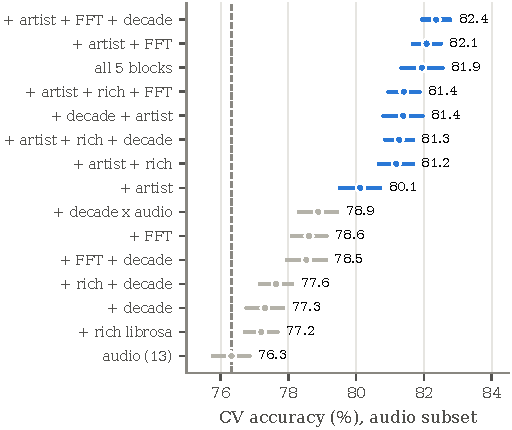
\includegraphics[width=\columnwidth]{fig_subset.pdf}
\caption{Every configuration evaluated on the 3{,}562-song audio subset, $5{\times}5$
cross-validated accuracy with 95\,\% CI, sorted. Blue: with artist history; gray: without.
Dashed line: the 13 Spotify descriptors alone.}
\label{fig:subset}
\end{figure}

% ---------------------------------------------------------------------
\subsection{Further experiments}\label{sec:further}

\textbf{Genre control for FFT.} We attach Spotify artist genres from the SpotGenTrack
release~\cite{martingutierrez2020multimodal} by normalised artist name (20{,}610 songs
with both a preview and a genre) and map the tags to 16 families. The benchmark's
construction is plainly visible: Latin, classical, jazz, ``world'' and metal artists
account for 50\,\% of the flops and 1.9\,\% of the hits, while rock, pop, R\&B,
hip-hop and country account for 93\,\% of the hits. Genre is also partly audible: a
Random Forest recovers the family from the 13 Spotify descriptors with 47.4\,\% accuracy,
from the 31 FFT descriptors with 49.9\,\% and from both with 53.3\,\% (majority class
26.1\,\%). Three results follow (Table~\ref{tab:genre}). (a) Genre families as features
raise the main model from $0.828$ to $0.928$ ($+10.1$\pp, 25/25, $p=8\times10^{-23}$):
on this benchmark, knowing the artist's genre is worth more than any audio
representation. (b) Once genre is known, FFT \emph{lowers} accuracy ($-1.1$\pp, 0/25,
$p=5\times10^{-7}$), also for new artists ($-1.4$\pp). (c) On a genre-matched sample
(as many hits as flops inside every family; 7{,}554 songs), FFT adds nothing to the main
model ($+0.1$\pp, 13/25, $p=0.84$; new artists $+0.1$\pp, $p=0.80$). FFT still improves
the 13 Spotify descriptors alone on that sample ($+2.5$\pp, 25/25, $p=5\times10^{-4}$),
but the main model, without FFT, still beats audio + FFT by $4.3$\pp{}
($p=2\times10^{-8}$). We conclude that the full-benchmark FFT gain is a genre shortcut,
whereas the gain of artist history survives the genre control. Spotify assigns artist
genres retrospectively, so we use them only as a control, never as a predictive feature.

\begin{table}[t]
\centering
\caption{Genre control for FFT ($5{\times}5$ CV). Left: songs with a preview and a Spotify
genre. Right: genre-matched sample. Accuracy overall and on songs by new artists.}
\label{tab:genre}
\setlength{\tabcolsep}{3pt}
\begin{tabular}{lcccc}
\toprule
& \multicolumn{2}{c}{All (20{,}610)} & \multicolumn{2}{c}{Matched (7{,}554)} \\
Model & Acc. & new art. & Acc. & new art. \\
\midrule
main (audio+decade+artist) & .828 & .780 & .790 & .749 \\
\quad + FFT & .841 & .798 & .791 & .750 \\
\quad + genre & .928 & .911 & -- & -- \\
\quad + genre + FFT & .917 & .897 & -- & -- \\
\midrule
FFT vs main, $\Delta$ ($p$) & \multicolumn{2}{c}{$+1.3$ ($10^{-4}$)} & \multicolumn{2}{c}{$+0.1$ (.84)} \\
FFT vs main+genre, $\Delta$ ($p$) & \multicolumn{2}{c}{$-1.1$ ($5\times10^{-7}$)} & \multicolumn{2}{c}{--} \\
\bottomrule
\end{tabular}
\end{table}

\textbf{Artist resolution.} The 52.1\,\% match rate is not a matching problem: 99.99\,\%
of the hits are found in the chart history up to their own decade, and the unmatched songs
are flops whose artists never charted (2.8\,\% of flops are matched). Two alternatives give
no gain: matching the full credited name before the primary artist (``Simon \&
Garfunkel'' rather than ``Simon'') lowers accuracy ($0.827$ vs $0.832$, $-0.5$\pp,
$p=4\times10^{-4}$), and crediting featured appearances changes nothing ($+0.1$\pp,
$p=0.39$). Canonical identifiers would avoid homonyms but cannot raise the match rate.

\textbf{How fast does a model age?} We train on a single decade and test on every later
one (Table~\ref{tab:decay}, songs with a preview). Audio-only accuracy falls from
$0.809$ within a decade to $0.765$ one decade later and $0.689$ three decades later.
Artist history slows the decay, and its advantage grows with the gap ($+2.8$\pp{} within
a decade, $+5.1$\pp{} three decades later). FFT behaves in the opposite way: it helps
within a decade ($+2.2$\pp) but hurts from three decades on, consistent with descriptors
that encode era-specific production and genre rather than lasting appeal. The cells
average 6 to 1 train/test pairs and are not tested for significance.

\begin{table}[t]
\centering
\caption{Rolling origin: train on one decade, test $k$ decades later (Random Forest,
35{,}370 songs with a preview; $k=0$: 5-fold CV inside each decade). Mean accuracy over
the available decade pairs.}
\label{tab:decay}
\setlength{\tabcolsep}{4pt}
\begin{tabular}{cccccc}
\toprule
$k$ & pairs & audio & + artist & + FFT & + artist + FFT \\
\midrule
0 & 6 & .809 & .837 & .831 & \textbf{.859} \\
1 & 5 & .765 & .796 & .782 & \textbf{.810} \\
2 & 4 & .728 & \textbf{.775} & .736 & \textbf{.775} \\
3 & 3 & .689 & \textbf{.740} & .673 & .728 \\
4 & 2 & .666 & \textbf{.734} & .661 & .718 \\
5 & 1 & .664 & \textbf{.754} & .599 & .706 \\
\bottomrule
\end{tabular}
\end{table}

\textbf{Lyrics on SpotGenTrack.} SpotGenTrack provides six lexical descriptors of the lyrics (syllables
per word, words per sentence, sentence count, word count, sentence similarity,
vocabulary richness) for 79{,}420 tracks with lyrics (21.5\,\% hits; $5{\times}1$ CV as in
Sec.~\ref{sec:external}). They improve the 13 Spotify descriptors (AUC $0.678\to0.729$,
$p=3\times10^{-4}$) and still add on top of decade and artist history (accuracy
$0.808\to0.814$, 5/5 folds, $p=0.002$; AUC $0.774\to0.797$, $p=2\times10^{-5}$). The gain
is modest in accuracy because of the class imbalance, and five folds are too few for it to
survive the Bonferroni correction, so we tested lyrics again on a larger, balanced dataset.

\subsection{Lyrics on ISMIR 2019}\label{sec:lyrics}
ISMIR songs are Million Song Dataset tracks, for which the official musiXmatch
release~\cite{bertinmahieux2011million} gives the lyrics of 237{,}662 tracks as word counts over the
5{,}000 most frequent (stemmed) words. Coverage is itself a shortcut: 56\,\% of the hits have lyrics against
36\,\% of the non-hit pool, so ``has lyrics'' would predict the label. We therefore keep only songs
\emph{with} lyrics on both sides and redraw balanced samples under protocols A and B. A second shortcut is
language: 97.5\,\% of the hits but only 80.5\,\% of the non-hits are mainly in English (at least 25\,\% of
their words among the 29 most common English words). We therefore also repeat every test on English songs
only. Two lyrics inputs are added to the final ISMIR model (audio + year + artist history): eight lexical
features (log number of words and of distinct words, richness, repetition, share of \emph{I/me/my},
\emph{you/your}, \emph{love} and of common English words), and one bag-of-words score, the out-of-fold
probability of a TF-IDF logistic regression trained inside each training fold, as for titles.

\begin{table}[t]
\centering
\caption{Lyrics on ISMIR 2019 (songs with lyrics only; Random Forest, $5{\times}2$ CV, corrected $t$-test
vs the final model of the same row; all rows 10/10 folds improved). Unseen: no artist in both training and
test folds.}
\label{tab:lyrics}
\footnotesize
\setlength{\tabcolsep}{2.6pt}
\begin{adjustbox}{max width=\columnwidth}
\begin{tabular}{@{}lccccc@{}}
\toprule
Sample & Songs & Final & + lyrics & $\Delta$ ($p$) & AUC \\
\midrule
A: random & 6{,}526 & .728 & \textbf{.775} & +4.7 ($3{\cdot}10^{-4}$) & .798$\to$.851 \\
B: year-matched & 6{,}478 & .676 & \textbf{.727} & +5.1 ($2{\cdot}10^{-5}$) & .732$\to$.802 \\
A, English & 6{,}364 & .718 & \textbf{.745} & +2.7 ($6{\cdot}10^{-4}$) & .788$\to$.820 \\
B, English & 6{,}294 & .658 & \textbf{.708} & +4.9 ($10^{-4}$) & .720$\to$.772 \\
A, English, unseen & 6{,}364 & .712 & \textbf{.742} & +3.0 ($6{\cdot}10^{-4}$) & .785$\to$.817 \\
B, English, unseen & 6{,}294 & .656 & \textbf{.700} & +4.4 ($3{\cdot}10^{-5}$) & .717$\to$.764 \\
\midrule
\multicolumn{6}{@{}l}{Lyrics alone (B, year-matched): .702, above the final model without lyrics (.676)} \\
\bottomrule
\end{tabular}
\end{adjustbox}
\end{table}

\begin{figure*}[t]
\centering
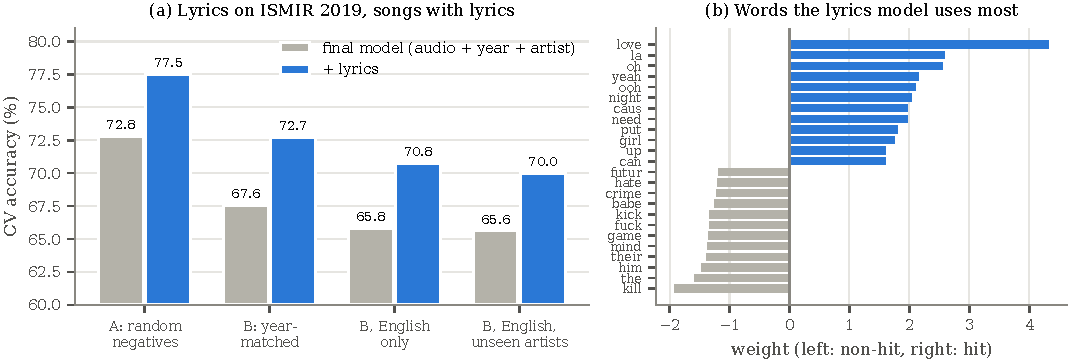
\includegraphics[width=\textwidth]{fig_lyrics.pdf}
\caption{Lyrics on ISMIR 2019. (a) Cross-validated accuracy of the final model without (gray) and with (blue)
the lyrics inputs, from the plain protocol to the strictest control (year-matched, English only, no artist in
both training and test folds). (b) Largest weights of the bag-of-words model fitted on the year-matched
English sample (stemmed words used in at least 30 songs; ``caus'' = cause, ``futur'' = future).}
\label{fig:lyrics}
\end{figure*}

Table~\ref{tab:lyrics} and Fig.~\ref{fig:lyrics}a show that lyrics add $+4.7$ points in protocol~A and
$+5.1$ in the year-matched protocol~B, in all 10 folds. The gain shrinks but remains when only English songs are
kept ($+2.7$ and $+4.9$), and it remains when, in addition, no artist appears in both training and test folds
($+3.0$ and $+4.4$, $p=3\times10^{-5}$; AUC $+0.047$, $p=10^{-6}$), so it does not come from recognising the
vocabulary of artists seen in training. These gains survive the Bonferroni correction. In the year-matched
protocol, lyrics alone (0.702) are more accurate than audio, year and artist history together (0.676).
Fig.~\ref{fig:lyrics}b shows what the model reads. Hit lyrics favour \emph{love} (by far the largest weight),
vocables (\emph{la}, \emph{oh}, \emph{ooh}, \emph{yeah}, \emph{hey}) and direct address (\emph{need},
\emph{girl}, \emph{night}). Non-hit lyrics favour darker or narrative words (\emph{kill}, \emph{hate},
\emph{crime}, \emph{mind}, \emph{their}, \emph{the}). On average, hit lyrics are slightly longer and use a
smaller share of distinct words (richness 0.34 vs 0.42), use \emph{love} twice as often (1.3\,\% vs 0.65\,\% of words) and
use \emph{you} more (5.5\,\% vs 4.6\,\%). These words point to themes and genres (romantic pop against metal,
punk or hardcore rap) as much as to style. On ISMIR this is a real difference between chart songs and the rest of
the catalogue rather than a construction rule, since the negatives are drawn at random. But it means that lyrics,
like genre, tell \emph{mainstream} songs from the rest more than they measure the appeal of an individual song.
We could not test lyrics on the Hit Predictor, whose songs have no Million Song Dataset identifier.

% ---------------------------------------------------------------------
\subsection{Time series: chart dynamics}\label{sec:timeseries}

\textbf{The chart as a time series.} The weekly Hot~100 (3{,}545 charts, 1958--2026) also
forms time series. The monthly mean number of debuts per chart week (1959--2025) is mostly
trend: an STL decomposition~\cite{cleveland1990stl} gives a trend strength of 0.72 and a
seasonal strength of 0.11~\cite{hyndman2021forecasting}. Debuts fall from 11.0 per week in
1959 to 5.5 in 2001 and return to 10.9 in 2025, after the chart started counting streams;
the largest residual is a rule change (60 debuts in the chart of 5 December 1998, when
songs not released as singles became eligible). The weekly number of holiday songs on the
chart is almost purely seasonal: its periodogram peaks at 52.1, 26.1, 17.4 and 13.0 weeks,
and a Fourier regression fitted on the streaming era ($K=20$ harmonics) explains 94\,\% of
its variance. Forecasting monthly debuts 12 months ahead under rolling-origin evaluation
(11 origins, 2015--2025), ARIMA$(1,1,2)$~\cite{box2015time} and ARIMA with Fourier terms
(MASE 1.82) and damped Holt-Winters (1.85) are best and indistinguishable ($p=0.97$); they
beat the seasonal naive forecast (2.32) at 10 of 11 origins ($p=0.006$). A seasonal ARIMA
(1.89) and gradient boosting or random forests on lag and Fourier features (1.94, 1.99) do
worse: the series has little seasonality, and 800 points leave tree models little to learn.

\textbf{Before release: market trends.} We describe each Hit Predictor song by the
distance of its standardised audio descriptors to the centroid of the previous decade's
hits, and by its projection on the direction in which that centroid moved. On top of the
main model these two features add $+0.07$\pp{} ($p=0.66$); the 13 per-feature deviations add
$+0.46$\pp{} (23/25, $p=0.006$). On audio alone the trend features add $+1.8$\pp{}
($p=7\times10^{-10}$), less than the decade alone ($+2.0$\pp): they carry era information,
which the main model already has.

\textbf{After release: early trajectories.} A different question can be asked once a song
has entered the chart: will it become a big hit? We take the 31{,}925 songs with a complete
history (debut after the first chart and at least 52 weeks of follow-up; 16.4\,\% reach
the top~10) and describe each by its first $k$ weeks on the chart. Concretely, ``the first
$k$ weeks'' are the $k$ chart positions the song holds in the $k$ weekly charts that start with
its debut: week~1 is the debut chart, week~2 the next week's chart, and so on, with position 101
if the song has dropped off. Madonna's \textit{Vogue}, for example, debuted at 39, then held 28
and 12 (so for $k=3$ the input is $(39, 28, 12)$) and later peaked at number~1. From these
positions we also compute the best rank so far, the average climb per week (slope), the change
of the weekly move (acceleration) and the number of weeks on the chart, and we add as context the
year, month, and the artist's earlier songs and earlier top-10 hits reached before the debut
(Random Forest, 200 trees, $5{\times}3$ CV). Table~\ref{tab:traj} shows that the trajectory dominates: three weeks give
an AUC of 0.892 against 0.593 for the context alone, and context adds $+0.03$ to $+0.05$ on
top (15/15 folds, $p<10^{-6}$ for every $k$). The prediction is not limited to songs already
at the top: among the songs not yet in the top~10 after three weeks, the AUC is 0.870, and a
model trained on songs before 2000 reaches 0.852 on songs from 2000 onwards. As for online
content~\cite{szabo2010predicting}, early popularity predicts later popularity. This task
differs from that of Sec.~\ref{sec:main}: every song has already charted, so it separates
big hits from small ones and cannot be used before release. A second target, at least
20~weeks on the chart, depends on chart rules that remove older songs and is not reported.

\textbf{What happens in the first three weeks.} Fig.~\ref{fig:traj} shows why so few weeks are
enough. Songs that will reach the top~10 already differ at their debut (median position 73 against
87), but the gap opens in the following weeks: their median position climbs to 53 in week~2 and 39
in week~3, while the other songs stay around 80 and one in four has already left the chart by
week~3 (Fig.~\ref{fig:traj}a). The climb matters as much as the starting point
(Fig.~\ref{fig:traj}b): a song that debuts between 61 and 80 and loses ground reaches the top~10
3\,\% of the time, but 55\,\% of the time if it climbs 30 places or more by week~3. Even among debuts in
the top~40, the share is 28\,\% for songs that fall and 82--100\,\% for songs that climb at least ten
places. Permutation importance of the $k=3$ model (Fig.~\ref{fig:traj}c, held-out AUC 0.893) confirms
this. Shuffling the week-3 position costs 0.088 AUC, the climb per week 0.029 and the best rank 0.025,
whereas the debut position alone costs 0.004 once the later weeks are known. Among the context inputs,
only the year matters (0.023), because chart dynamics changed over time; the artist's earlier songs cost
less than 0.01. After release, then, it is the song's own momentum, not the artist's past, that tells a big
hit from a small one.

\begin{figure*}[t]
\centering
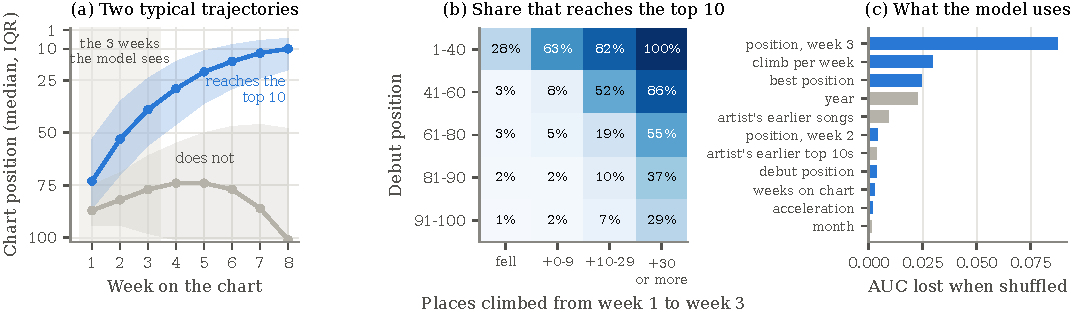
\includegraphics[width=\textwidth]{fig_traj.pdf}
\caption{The first weeks on the Hot~100 (31{,}925 songs, 5{,}238 reach the top~10). (a) Median chart
position (line) and interquartile range (band) in each week after the debut; 101 = off the chart. The
shaded weeks are the inputs of the $k=3$ model. (b) Share of songs that eventually reach the top~10, by
debut position and by places gained between week~1 and week~3 (``fell'': lost places or left the chart).
(c) Permutation importance of the inputs of the $k=3$ model on a held-out 25\,\%: drop in ROC-AUC when one
input is shuffled. Blue: trajectory; gray: context.}
\label{fig:traj}
\end{figure*}

\begin{table}[t]
\centering
\caption{Predicting a top-10 peak from a song's first $k$ weeks on the Hot~100 (31{,}925
songs, 16.4\,\% top-10; Random Forest, $5{\times}3$ CV). Context: year, month and the
artist's earlier chart history. Last column: songs not yet in the top~10 after $k$ weeks.}
\label{tab:traj}
\setlength{\tabcolsep}{4pt}
\begin{tabular}{ccccc|c}
\toprule
 & \multicolumn{4}{c|}{All songs} & Not yet top 10 \\
$k$ & weeks & + context & F1 & context only & + context \\
\midrule
1 & .700 & .750 & .401 & .593 & .720 \\
2 & .796 & .850 & .531 & .593 & .828 \\
3 & .845 & \textbf{.892} & .610 & .593 & .870 \\
4 & .891 & \textbf{.917} & .674 & .593 & .894 \\
\bottomrule
\end{tabular}
\end{table}

% =====================================================================
\section{Discussion}\label{sec:discussion}

\textbf{The final model.} After the audit, the model we retain is the main model of
Sec.~\ref{sec:main}: the frozen Random Forest (80 trees, 8 candidate features per split) on 20
inputs per song, namely the 13 Spotify descriptors, six decade indicators and artist history
$h(s)$. It reaches 0.832 accuracy and 0.918 ROC-AUC on the Hit Predictor
(Table~\ref{tab:main}). On the external datasets the same recipe is used with each dataset's
own audio descriptors, the release year or decade and artist history, with a 200-tree Random
Forest (0.763 on ISMIR protocol~A, 0.708 on protocol~B, ROC-AUC 0.777 on SpotGenTrack).
XGBoost is 1.3 points more accurate under cross-validation but ties with the Random Forest on
the canonical split ($p=0.87$), so we keep the configuration that matches prior work. Every
other candidate is left out for a stated reason (Table~\ref{tab:final}). A separate model
answers a different question, for songs already on the chart: the same kind of Random Forest
on the first weeks of the chart trajectory (Sec.~\ref{sec:timeseries}). Where lyrics are available
(ISMIR, songs with musiXmatch lyrics), adding them gives the best model we found on that dataset (0.775 in
protocol~A, 0.727 in protocol~B; Table~\ref{tab:lyrics}).

\begin{table}[t]
\centering
\caption{Inputs of the final model. Gains in accuracy points over the 13 Spotify
descriptors on the Hit Predictor ($5{\times}5$ CV) unless stated.}
\label{tab:final}
\footnotesize
\setlength{\tabcolsep}{3pt}
\begin{tabular}{@{}>{\raggedright\arraybackslash}p{2.75cm}>{\raggedright\arraybackslash}p{1.75cm}>{\raggedright\arraybackslash}p{3.15cm}@{}}
\toprule
Input & Evidence & Decision \\
\midrule
13 Spotify descriptors & 0.782 & kept (baseline) \\
Decade (6 indicators) & $+2.0$ & kept; helps new artists \\
Artist history $h(s)$ & $+2.9$; ISMIR~B $+2.6$ & kept; survives every control \\
\midrule
Song title (TF-IDF) & $+6.7$ & out: construction artefact \\
Title length & $+0.2$, n.s. & out: no signal \\
chorus\_hit, sections & $0.0$, n.s. & out: no signal \\
Rich librosa (PCA 40) & $+0.9$, n.s. & out: single-split luck \\
FFT (31) & $+0.1$ genre-matched & out: genre shortcut \\
Spotify artist genre & $+10.1$ & control only: assigned afterwards \\
Market trend & $+0.07$, n.s. & out: carries only the era \\
Lyrics (bag of words + 8 lexical) & ISMIR~B $+4.4$, unseen artists & kept where lyrics exist (ISMIR); unavailable for the Hit Predictor \\
\bottomrule
\end{tabular}
\end{table}

\textbf{How much of the gain is real?} The benchmark's negative class excludes the artists
of that decade's hits. Our feature only counts \emph{earlier} decades, so it is leakage-free
in time, but an artist who charted before is likely to chart again and is therefore
unlikely to appear as a negative by construction: flops have on average 0.037 earlier hits,
against 3.21 for hits. The $+5.0$\pp{} on this benchmark, and the head-to-head gains of
Table~\ref{tab:tilburg}, should be read as benchmark-specific. The ISMIR year-matched
protocol, whose negatives are chosen neither by artist nor by date, gives a more
conservative $+2.6$\pp; this is the number we consider transferable.

\textbf{Era as a shortcut.} On ISMIR, release year looks like a strong predictor (70.2\,\%
alone, and $+12$--$13$\,\% in the original study) because hits are older than the
non-hit pool. Once years are matched, it carries no information. On the Hit Predictor, the
decade is uninformative alone and helps only through interactions, which is consistent
with era-specific tastes but may also reflect decade-dependent genre rules of the negative
class. Reported gains from date features should be accompanied by a year-matched control.

\textbf{Genre as a shortcut.} On the Hit Predictor, the artist's genre alone takes the
main model to $0.928$, and the apparent FFT gain disappears once genre is controlled
(Sec.~\ref{sec:further}). Any audio representation evaluated on this benchmark can score
by recognising the excluded genres rather than by modelling what makes a song a hit, so
audio gains on it should be reported together with a genre-matched control. Artist history
passes that control; FFT does not. Within the audio content itself, therefore, no
representation we tested adds to artist history and era once the construction shortcuts
are controlled. The one content input that does is the lyrics (Sec.~\ref{sec:lyrics}), whose
gain survives year matching, an English-only control and unseen artists; their strongest words,
however, suggest that they too partly identify mainstream genres and themes. On these data, what
predicts a hit is mostly who sings it, when, and what the song is about---not how it sounds.

\textbf{Single splits mislead.} Several conclusions of our own earlier single-split
analysis did not survive cross-validation. With a few thousand songs, an 891-song test set
has a standard error of about 1.4\pp, so single-split gains of 3--4\pp{} on subsets are
fragile even when McNemar's test is significant on that split.

\begin{table*}[t]
\centering
\caption{Survival ranking: every tested gain, ranked by how far it survives. A gain \emph{survives} if it is
significant under cross-validation, remains significant after the Bonferroni correction over the $\approx$\,60
tests of the paper ($p<8\times10^{-4}$), and passes the control that removes the known shortcut of its dataset.
$\Delta$: accuracy points unless stated; $p$: corrected $t$-test (McNemar for single splits).}
\label{tab:survival}
\footnotesize
\setlength{\tabcolsep}{3.5pt}
\begin{tabular}{@{}l>{\raggedright\arraybackslash}p{5.1cm}rrcc>{\raggedright\arraybackslash}p{4.3cm}@{}}
\toprule
& Gain tested & $\Delta$ & $p$ & Bonf. & Control & Verdict \\
\midrule
\multirow{12}{*}{\rotatebox{90}{\textbf{survived (low $p$)}}}
& Decade + artist history, Hit Predictor & +5.0 & $7{\cdot}10^{-17}$ & \checkmark & \checkmark & real; benchmark-inflated (unseen artists: +5.0, $10^{-13}$) \\
& Every classifier, decade + artist (5 models) & +4.6 to +5.7 & $\leq 4{\cdot}10^{-5}$ & \checkmark & \checkmark & gain comes from the inputs, not the model \\
& Head-to-head, Du's models + artist (6 settings) & +2.1 to +3.2 & $\leq 6{\cdot}10^{-6}$ & \checkmark & \checkmark & better on 50/50 splits \\
& Future decades, artist history (3 decades) & +1.9 to +3.4 & $\leq 10^{-7}$ & \checkmark & \checkmark & survives a temporal shift \\
& Decade, Hit Predictor & +2.0 & $10^{-10}$ & \checkmark & \checkmark & helps new artists (+2.2, $2{\cdot}10^{-9}$) \\
& Artist history, ISMIR A (vs audio) & +2.5 & $2{\cdot}10^{-5}$ & \checkmark & \checkmark & real \\
& Artist history, ISMIR B year-matched & +2.6 & $3{\cdot}10^{-5}$ & \checkmark & \checkmark & \textbf{transferable estimate}; unseen artists +2.9 ($9{\cdot}10^{-7}$) \\
& Decade + artist, SpotGenTrack (AUC .690$\to$.777) & +1.3 & $3{\cdot}10^{-4}$ & \checkmark & \checkmark & F1 .147$\to$.358 ($7{\cdot}10^{-7}$) \\
& Lyrics, ISMIR B, English, unseen artists & +4.4 & $3{\cdot}10^{-5}$ & \checkmark & \checkmark & only content input that survives \\
& Lyrics, ISMIR A, English, unseen artists & +3.0 & $6{\cdot}10^{-4}$ & \checkmark & \checkmark & same, weaker \\
& Early trajectory, 3 weeks + context vs weeks (AUC) & +.047 & $<10^{-6}$ & \checkmark & \checkmark & after release only; AUC 0.892 \\
& Genre-control results (FFT given genre) & $-1.1$ & $5{\cdot}10^{-7}$ & \checkmark & -- & shows that FFT encodes genre \\
\midrule
\multirow{4}{*}{\rotatebox{90}{\textbf{shortcut}}}
& Song title (TF-IDF), Hit Predictor & +6.7 & $4{\cdot}10^{-20}$ & \checkmark & $\times$ & artefact of how non-hits were collected \\
& Spotify artist genre, Hit Predictor & +10.1 & $8{\cdot}10^{-23}$ & \checkmark & $\times$ & not known on release day; control only \\
& FFT, whole Hit Predictor & +1.4 & $4{\cdot}10^{-9}$ & \checkmark & $\times$ & genre-matched: +0.1 ($p=0.84$) \\
& Release year, ISMIR A & +3.1 & $2{\cdot}10^{-4}$ & \checkmark & $\times$ & year-matched: $-0.1$ ($p=0.66$) \\
\midrule
\multirow{11}{*}{\rotatebox{90}{\textbf{did not survive (high $p$)}}}
& Lyrics lexical, SpotGenTrack ($5{\times}1$) & +0.6 & .002 & $\times$ & -- & indicative; confirmed on ISMIR \\
& Market trend, 13 per-feature deviations & +0.46 & .006 & $\times$ & -- & indicative only \\
& ARIMA vs seasonal naive (11 origins) & MASE $-0.5$ & .006 & $\times$ & -- & indicative only \\
& FFT on top of artist, audio subset & +2.0 & .008 & $\times$ & $\times$ & genre shortcut (see above) \\
& Decade, audio subset & +1.0 & .03 & $\times$ & -- & small sample \\
& Audio + artist + FFT vs final, whole benchmark & +0.4 & .04 & $\times$ & $\times$ & no \\
& Rich librosa (PCA 40), audio subset & +0.9 & .15 & $\times$ & -- & single split said +3.8 ($p=.002$) \\
& Artist history for new artists, Hit Predictor & +0.4 & .17 & $\times$ & -- & cannot help: $h(s)=0$ \\
& Title length & +0.2 & .28 & $\times$ & -- & no signal \\
& Market trend, distance + direction & +0.07 & .66 & $\times$ & -- & carries only the era \\
& \texttt{chorus\_hit} + \texttt{sections} & 0.0 & .82 & $\times$ & -- & no signal \\
\bottomrule
\end{tabular}
\end{table*}

\textbf{Survival ranking.} Table~\ref{tab:survival} lists every gain we tested, split into three groups.
\emph{Survived}: low $p$ after Bonferroni and passing the control of its dataset. \emph{Shortcut}: low $p$
but failing the control, so the gain is real on that dataset but would not transfer. \emph{Did not survive}:
high $p$ (above the Bonferroni threshold). Only artist history, era, the lyrics and, after release, the early
trajectory are in the first group.

\textbf{Multiple comparisons.} The paper reports about 60 $p$-values without correction for
multiplicity. Every result our conclusions rest on remains significant after a Bonferroni
correction over all of them ($p < 0.05/60 \approx 8\times10^{-4}$): the main gains of
Tables~\ref{tab:main} and~\ref{tab:models}, the head-to-head of Table~\ref{tab:tilburg},
the temporal hold-out, the ISMIR gains of artist history in both protocols, and the
artist-grouped gains. The full-benchmark FFT gain on top of the main model also survives
($p=4\times10^{-9}$) but is explained by genre (Sec.~\ref{sec:further}); the genre-control
results themselves ($p\leq5\times10^{-7}$) survive as well, and so do the early-trajectory
gains of Table~\ref{tab:traj} ($p<10^{-6}$). Results with $8\times10^{-4} < p < 0.05$ should be read as
indicative only: the decade and FFT gains on the 3{,}562-song audio subset (including FFT
on top of artist history), audio + artist + FFT against the main model on the whole
benchmark ($p=0.04$), the per-feature market-trend deviations ($p=0.006$), the
forecasting comparison of Sec.~\ref{sec:timeseries} ($p=0.006$, 11 origins), the lyrics gains on SpotGenTrack ($5{\times}1$ CV, $p=0.002$ for
accuracy; the ISMIR lyrics gains, $p\leq6\times10^{-4}$, survive), most single-split gains on
that subset, the SpotGenTrack accuracy gain of artist history alone ($p=10^{-3}$; with
decade, $p=3\times10^{-4}$), and the ISMIR cold-start gains of artist history for known
artists in protocol A and new artists in protocol B.

\textbf{Limitations.} Artist history is matched by normalised name, not by a canonical
identifier, so homonymous artists can be merged. Artist history does not help new artists on
the Hit Predictor and helps them only modestly on ISMIR ($+1.4$\pp), and it partly measures
cumulative advantage~\cite{salganik2006experimental} rather than the intrinsic appeal
of a song. We use classical classifiers on fixed descriptors rather than deep networks on
raw audio~\cite{yang2017revisiting,nofer2026deephits}: our question is which inputs carry
signal under a controlled protocol, and the comparison with prior work is made at equal
model; a learned representation could still capture what the descriptors miss. The
comparison with Zangerle et~al.\ uses a classifier rather than their regression on chart
position and a different random draw of negatives; the comparison with Du uses re-drawn
splits. Our audio previews are 30-second clips from a different service than the one that
computed the Spotify descriptors.

% =====================================================================
\section{Future Work}

Sec.~\ref{sec:further} already runs the cheap versions of several follow-ups: artist
matching (no gain available), a genre control for audio features, rolling-origin decay and
lexical lyrics descriptors. What remains needs new data.
(i) \emph{Cold start}: artist history barely helps first-time artists on the benchmark, and
the FFT gain for them was a genre shortcut; features such as label, collaborators, prior
streams or social media remain to be tested, with a genre-matched control.
(ii) \emph{Lyrics and emotion}: lyrics for the Hit Predictor songs (matched by title and
artist), a genre-matched control for the lyrics gain, semantic and affective lyrics representations, and learned
audio embeddings, evaluated with the same audit protocol.
(iii) \emph{Benchmark design}: a hit-prediction dataset whose negatives are sampled
independently of artist, genre and date. Our genre-matched sample is a small, post-hoc
approximation of it; a purpose-built one would let content features be compared without
construction shortcuts.
(iv) \emph{Early trajectories}: Sec.~\ref{sec:timeseries} uses weekly chart positions only;
daily streams and radio plays would allow the same prediction days after release.

\section{Conclusion}
A song's artist history is a simple, leakage-free signal that improves hit prediction
across classifiers, beats the only prior model on the Spotify Hit Predictor benchmark in a
head-to-head comparison, and transfers to an independent peer-reviewed dataset where it
exceeds the best published accuracy and survives a year-matched control. These gains hold
for artists the model never saw in training, which rules out artist recognition; but artist
history cannot help an artist with no earlier hit, and for those newcomers only era context helps; spectral descriptors of a 30-second
preview appear to help them too, but that gain disappears under a genre control. The same audit
shows that larger gains---song titles, release dates, genre-driven audio features, rich
audio on a single split---can
come from how the data were built or from chance. Chart time series add nothing before
release, but after release a song's first weeks are the strongest predictor we found. The lyrics are
the only content input whose gain survives every control. Knowing which gains are real matters more
than the headline number.

\section*{Code and data availability}
\textbf{Code.} \url{\repourl}. Every number in this paper is produced by the scripts in
\texttt{repro/} (shared data loading and evaluation in \texttt{common.py}; one script per
section, Table~\ref{tab:scripts}) and written to \texttt{paper\_results/}. Random seeds are fixed (42 unless
stated). \texttt{docs/DATA.md} explains where each dataset goes.

\textbf{Data.} All datasets are public:
Spotify Hit Predictor~\cite{ansari2020dataset}, \url{https://github.com/fortyTwo102/The-Spotify-Hit-Predictor-Dataset}
(also Kaggle: \url{https://www.kaggle.com/datasets/theoverman/the-spotify-hit-predictor-dataset});
Billboard Hot~100 weekly charts, \url{https://github.com/utdata/rwd-billboard-data};
ISMIR~2019 hit-song data~\cite{zangerle2019hit}, \url{https://zenodo.org/records/3258042};
SpotGenTrack~\cite{martingutierrez2020multimodal}, \url{https://data.mendeley.com/datasets/4m2x4zngny};
musiXmatch lyrics for the Million Song Dataset, \url{http://millionsongdataset.com/musixmatch/}.
Audio previews were retrieved from the public Deezer API (\url{https://developers.deezer.com/api}).

% =====================================================================
\appendices

\section{Inputs in detail}\label{app:inputs}

\begin{table}[h]
\centering
\caption{The 13 Spotify audio descriptors (Spotify Web API definitions) and how well each one alone
separates hits on the Hit Predictor (ROC-AUC; Sec.~\ref{sec:ablation}).}
\label{tab:descriptors}
\footnotesize
\setlength{\tabcolsep}{3pt}
\begin{tabular}{@{}l>{\raggedright\arraybackslash}p{4.6cm}c@{}}
\toprule
Descriptor & Meaning & AUC \\
\midrule
instrumentalness & likelihood that the track has no vocals (0--1); lower in hits & .74 \\
danceability & suitability for dancing from tempo, rhythm stability, beat strength (0--1) & .70 \\
loudness & average loudness in dB & .64 \\
valence & musical positiveness, sad (0) to happy (1) & .64 \\
acousticness & confidence that the track is acoustic (0--1); lower in hits & .60 \\
energy & perceived intensity and activity (0--1) & .59 \\
speechiness & presence of spoken words (0--1) & .58 \\
mode & major (1) or minor (0) & .54 \\
time signature & estimated beats per bar & .53 \\
liveness & probability that the track was recorded live & .53 \\
tempo & estimated beats per minute & .52 \\
duration & length in milliseconds & .51 \\
key & pitch class of the track (0 = C, \dots, 11 = B) & .51 \\
\bottomrule
\end{tabular}
\end{table}

\textbf{Decade.} Six indicators (1960s \dots\ 2010s), exactly one equal to 1. On ISMIR and SpotGenTrack,
the release year (or decade) as a number.

\textbf{Artist history.} Defined in Sec.~\ref{sec:features} and Fig.~\ref{fig:history}. Artist names are
lower-cased, accents and punctuation are removed, and only the first credited artist is kept
(the name is cut at ``featuring'', ``feat.'', ``ft.'', ``with'', ``\&'', ``x'', ``+'', ``/'', ``vs.'',
``and'' or a comma), so that ``Madonna feat.\ Justin Timberlake'' counts for Madonna.
On the Hit Predictor the reference set is the weekly Hot~100 since August 1958, counted in distinct
titles per artist and decade; on ISMIR and SpotGenTrack it is the set of positive songs of the dataset,
counted by release year.

\textbf{Rejected candidates.} \emph{Song title}: TF-IDF of word uni- and bigrams, logistic regression,
out-of-fold probability as one feature. \emph{Title length}: number of words. \emph{chorus\_hit,
sections}: the two Echo Nest analysis fields of the Hit Predictor. \emph{Rich librosa} (185): 20 MFCCs
with first and second derivatives, chroma, tonnetz, spectral contrast, centroid, bandwidth, roll-off,
flatness, zero-crossing rate, RMS and onset/tempogram statistics, each by mean and standard deviation,
reduced to 40 principal components inside each fold. \emph{FFT} (31): from the short-time Fourier transform of the 30-second clip, the mean and standard
deviation of the spectral centroid, bandwidth, roll-off, flatness and contrast, 13 mean MFCCs, the chroma mean
and standard deviation, and six rhythm descriptors (estimated tempo, onset-envelope mean and standard
deviation, pulse clarity, mean and variation of inter-onset intervals).
\emph{Genre} (16 families, control only): Spotify artist tags mapped by keyword to hip-hop, R\&B/soul,
country, rock, metal, electronic, pop, jazz, classical, folk, blues, Latin, reggae, gospel, world, other.
\emph{Market trend}: distance of the standardised descriptors to the previous decade's hit centroid,
projection on the direction in which that centroid moved, and the 13 per-descriptor deviations.

\textbf{Lyrics} (ISMIR). From musiXmatch word counts: log number of words, log number of distinct words,
richness (distinct/total), repetition (count of the most frequent word/total), shares of \emph{I, me,
my}, of \emph{you, your}, of \emph{love}, and of the 29 most common English words; plus the out-of-fold
TF-IDF logistic-regression probability.

\textbf{Early trajectory.} For $k$ weeks: the $k$ positions (101 = off the chart), the best position, the
number of weeks on the chart, the slope $(p_k-p_1)/(k-1)$ (negative = climbing), the acceleration
$(p_k-p_{k-1})-(p_{k-1}-p_{k-2})$; context: debut year and month, $\log(1+{}$earlier songs of the
artist$)$ and $\log(1+{}$earlier top-10 hits that had already reached the top~10 before the debut$)$.

\section{Models and settings}\label{app:models}

\begin{table}[h]
\centering
\caption{Every model used, with all non-default settings. None was tuned on the test data.}
\label{tab:settings}
\footnotesize
\setlength{\tabcolsep}{3pt}
\begin{tabular}{@{}>{\raggedright\arraybackslash}p{2.4cm}>{\raggedright\arraybackslash}p{5.6cm}@{}}
\toprule
Model & Settings \\
\midrule
Random Forest (main) & 80 trees, 8 candidate features per split, Gini, fully grown trees, seed 42 (configuration of~\cite{middlebrook2019song}) \\
Random Forest (external, trajectories) & 200 trees, $\sqrt{d}$ candidate features per split \\
XGBoost & 400 trees, depth 6, learning rate 0.05, subsample 0.8, column sample 0.8 \\
Logistic regression & standardised inputs, L2, $C=1$ \\
$k$-NN & standardised inputs, $k=25$ \\
SVM & standardised inputs, RBF kernel, $C=1$, $\gamma$ = scale \\
Du's models~\cite{du2022spotify} & RF 450 trees, $m_{\text{try}}=2$, at most 30 leaves; logistic regression; one model per decade \\
Title / lyrics text model & TF-IDF + logistic regression ($C=4$ titles, $C=1$ lyrics), inner 5-fold out-of-fold \\
Rich audio & standardisation + PCA (40) fitted inside each training fold \\
\midrule
Cross-validation & repeated stratified $k$-fold: $5{\times}5$ (Hit Predictor), $5{\times}2$ (ISMIR), $5{\times}1$ (SpotGenTrack), $5{\times}3$ (trajectories); stratified group $k$-fold by artist for the unseen-artist tests \\
Tests & corrected resampled $t$-test~\cite{nadeau2003inference} for CV; McNemar~\cite{dietterich1998approximate} for single splits; Bonferroni over $\approx$\,60 tests \\
\bottomrule
\end{tabular}
\end{table}

\FloatBarrier
\section{Extended related work}\label{app:related}

\textbf{Audio-based hit prediction.} Pachet and Roy~\cite{pachet2008hit} found that
acoustic and human-annotated descriptors could not predict popularity, while Ni
et~al.~\cite{ni2011hit} and Herremans et~al.~\cite{herremans2014dance} reported
above-chance results on chart data. Yang et~al.~\cite{yang2017revisiting} revisited the
problem with convolutional networks on audio. Zangerle et~al.~\cite{zangerle2019hit}
combined low- and high-level Essentia descriptors~\cite{bogdanov2013essentia} of Million
Song Dataset tracks~\cite{bertinmahieux2011million} in a wide-and-deep network and reached
75.04\,\% accuracy on a balanced set of 11{,}664 songs (5{,}832 hits; one is lost to a missing year or
incomplete descriptors, so we keep 5{,}831, App.~\ref{app:data}), noting that adding the release year
improved every configuration.

\textbf{Artist reputation.} Interiano et~al.~\cite{interiano2018musical} analyse more
than 500{,}000 UK songs (1985--2015) and show that a superstar indicator improves the
prediction of chart success over acoustic features alone. Salganik
et~al.~\cite{salganik2006experimental} showed experimentally that success in cultural
markets depends on social influence and cumulative advantage, which is one reason why an
artist's past success predicts future success.

\textbf{Spotify descriptors and Billboard labels.} Middlebrook and
Sheik~\cite{middlebrook2019song} matched about 24{,}000 Spotify tracks (1985--2018) to the
Hot~100 and reported 87.7\,\% test accuracy with a Random Forest; their feature list
includes chart-derived fields and an artist past-performance feature. SpotHitPy~\cite{dimolitsas2023spothitpy}
reported about 86\,\% on roughly 18{,}500 songs. Zhao et~al.~\cite{zhao2023analysis}
added engineered metadata and lyrics features for Top-10 prediction (89.1\,\% with a
Random Forest). These numbers come from different datasets and label definitions.
The Spotify Hit Predictor dataset~\cite{ansari2020dataset} is a public benchmark of
decade-balanced hits and non-hits (1960--2019); the only academic study we found on it is
an MSc thesis by Du~\cite{du2022spotify}, which reports 84\,\% (2000s) and 82\,\% (2010s)
with one Random Forest per decade.

\textbf{Multimodal and popularity prediction.} Mart\'in-Guti\'errez
et~al.~\cite{martingutierrez2020multimodal} released SpotGenTrack and predicted Spotify
popularity with an end-to-end multimodal network; DeepHits~\cite{nofer2026deephits}
combines log-Mel CNNs, lyric embeddings, artist popularity and release year on the same
data; Rompolas et~al.~\cite{rompolas2024predicting} use social-media sentiment.

\textbf{Evaluation pitfalls.} Dietterich~\cite{dietterich1998approximate} recommends
McNemar's test for a single split, and Nadeau and Bengio~\cite{nadeau2003inference} show
that naive $t$-tests over overlapping resamples are anti-conservative and propose a
corrected variance. Leakage~\cite{kaufman2012leakage} and shortcut
learning~\cite{geirhos2020shortcut} describe models that exploit cues unrelated to the
intended task. In music information retrieval, Sturm~\cite{sturm2014simple} showed that
systems can reach high scores through confounds in the ground truth (``horses''), and
Flexer~\cite{flexer2007closer} showed that letting songs by the same artist appear in
training and test sets inflates genre-classification accuracy; our artist-grouped
cross-validation applies this artist filter to hit prediction. To our knowledge, no hit-prediction study on Spotify descriptors reports
both a significance-tested head-to-head on the same data and an audit of construction
artefacts.

\FloatBarrier
\section{Datasets in detail}\label{app:data}

\textbf{Spotify Hit Predictor.} Six decade files (1960s--2010s) list 13 Spotify audio
descriptors (danceability, energy, key, loudness, mode, speechiness, acousticness,
instrumentalness, liveness, valence, tempo, duration, time signature), two analysis
fields (\texttt{chorus\_hit}, \texttt{sections}), the artist, the title and a binary
target~\cite{ansari2020dataset}. The six files hold 41{,}106 rows; 537 track URIs (App.~\ref{app:glossary})
appear more than once, 450 of them in two decade files and 26 with different labels. We keep the first copy in the
order the files are read (00s, 10s, 60s, 70s, 80s, 90s, i.e.\ alphabetical), which leaves 40{,}560 songs; a
song's decade is the decade of the file that copy comes from. A song is a hit if it appeared on the weekly Hot~100 in that decade. Crucially,
the dataset documentation states that a non-hit must satisfy all of: the track is not in
that decade's hit list, \emph{its artist is not in that decade's hit list}, it belongs to a
``non-mainstream and/or avant-garde'' genre, and that genre has no song in the hit list.
Each decade file is therefore balanced (48.3--49.9\,\% hits), and the negative class is
selected partly \emph{by artist} and \emph{by genre}. We return to this in
Sec.~\ref{sec:discussion}.

\textbf{Audio subset.} We first drew a random sample of 3{,}996 songs, the same number (333) in each of
the 12 decade $\times$ hit/non-hit cells (seed 42), and searched each one on the public Deezer API with the
query \texttt{artist:"<artist>" track:"<title>"} (the raw artist and title fields of the dataset, with double quotes
and backslashes removed), keeping the 30-second preview of the first result (the
quoted fields make Deezer require both the artist and the title; the match is not checked further, so a few
previews may be another version of the song). 3{,}562 songs
had a preview and complete descriptors; this is the \emph{audio subset}. The same search was later run on every
song (35{,}370 found, App.~\ref{sec:audit}). From the previews we extracted 31 spectral/rhythmic descriptors (``FFT'') and 185 richer
librosa~\cite{mcfee2015librosa} descriptors (20 MFCCs and their first and second
derivatives, chroma, tonnetz, spectral contrast, centroid, bandwidth, roll-off, flatness,
zero-crossing rate, RMS and onset/tempogram statistics, each summarised by mean and
standard deviation).

\textbf{ISMIR 2019.} The release of Zangerle et~al.~\cite{zangerle2019hit} provides
Essentia low- and high-level descriptors for 5{,}832 Hot~100 hits and 89{,}235 non-hits
from the Million Song Dataset, in two files (\texttt{msd\_bb\_matches.csv}, \texttt{msd\_bb\_non\_matches.csv}) that
give for each track its MSD identifier, artist, title and release year (from the MSD metadata). Tracks with a
missing or zero year are removed. On ISMIR the artist name is only lower-cased and trimmed (no accent or
featuring removal). We flatten all numeric descriptors of the Essentia JSON files: numbers are kept, lists of
numbers are summarised by their mean, while booleans, strings, lists of lists, the whole \texttt{metadata} block
(bit rate, codec, \dots) and the beat positions in seconds are skipped; we then keep the columns present for more
than 95\,\% of the tracks (computed over all tracks with descriptors: the hits and the whole non-hit pool), giving 592, drop every track with a missing value in one of them (no imputation),
keep the 5{,}831 hits with complete
descriptors and, like the original study, draw an equal number of non-hits (protocol A, 11{,}662 songs). The
year-matched sample of protocol B also has 11{,}662 songs. Hits have a median release year of 1987 and non-hits of 2001, a fact that matters
below.

\textbf{SpotGenTrack.} 101{,}909 Spotify tracks with 13 descriptors, 207 pre-extracted
low-level audio features and a popularity score~\cite{martingutierrez2020multimodal}; we
label tracks with popularity $\geq 55$ as hits (19.4\,\%). Because the classes are
imbalanced, we report ROC-AUC alongside accuracy for this dataset.

A fourth candidate, a Billboard year-end chart file (2000--2023) augmented with Spotify
features, was discarded: 2{,}911 of its 3{,}397 rows have no audio descriptors.

\FloatBarrier
\section{Main result: more detail}\label{app:main}
\begin{table}[!htbp]
\centering
\caption{Cross-validated accuracy per decade: the models of Table~\ref{tab:main}, trained on all decades in each
of the 25 folds, scored separately on the test songs of each decade (Random Forest).}
\label{tab:decade}
\footnotesize
\setlength{\tabcolsep}{3.2pt}
\begin{adjustbox}{max width=\columnwidth}
\begin{tabular}{@{}lcccccc@{}}
\toprule
Features & 60s & 70s & 80s & 90s & 00s & 10s \\
\midrule
Audio (13) & .743 & .750 & .770 & .806 & .836 & .816 \\
+ decade & .764 & .763 & .794 & .840 & .851 & .833 \\
+ artist & .763 & .784 & .812 & .831 & .860 & .842 \\
+ decade + artist & \textbf{.788} & \textbf{.796} & \textbf{.836} & \textbf{.864} & \textbf{.873} & \textbf{.868} \\
\bottomrule
\end{tabular}
\end{adjustbox}
\end{table}

The improvement holds in every decade (Table~\ref{tab:decade}), from $+3.7$\pp{} in the
2000s to $+6.6$\pp{} in the 1980s. Since each decade file is balanced, the decade indicator
carries no information on its own; its gain can only come from interactions with the audio
descriptors, i.e.\ from era-specific decision rules.

\begin{table}[!htbp]
\centering
\caption{Robustness to the classifier (5-fold CV with one repeat, $5{\times}1$, corrected $t$-test; all 5 folds
improve).}
\label{tab:models}
\footnotesize
\setlength{\tabcolsep}{3pt}
\begin{adjustbox}{max width=\columnwidth}
\begin{tabular}{@{}lcccc@{}}
\toprule
Classifier & Audio (13) & + decade + artist & $\Delta$ & $p$ \\
\midrule
Random Forest~\cite{breiman2001random} & .780 & .832 & +5.2 & $2{\cdot}10^{-5}$ \\
XGBoost~\cite{chen2016xgboost} & .788 & \textbf{.845} & +5.7 & $3{\cdot}10^{-7}$ \\
Logistic regression & .727 & .782 & +5.5 & $4{\cdot}10^{-5}$ \\
$k$-NN ($k=25$) & .750 & .796 & +4.6 & $8{\cdot}10^{-6}$ \\
SVM (RBF) & .773 & .828 & +5.5 & $3{\cdot}10^{-5}$ \\
\bottomrule
\end{tabular}
\end{adjustbox}
\end{table}

\textbf{Robustness to the classifier.} The gain is of the same size for five classifiers of
very different nature (Table~\ref{tab:models}), so it comes from the features rather than
from the model. XGBoost is the strongest on average, but on the canonical split it ties with
the frozen Random Forest (0.820 vs 0.822, McNemar $p=0.87$). TreeSHAP attributions of the
XGBoost model rank artist history first (mean $|\phi|=1.08$), the six decade indicators
second (0.86 summed) and instrumentalness third (0.73), ahead of every other descriptor.

\textbf{Future decades.} To test whether the gain survives a temporal shift, we train on all
earlier decades and test on a later one, with no song from the test decade seen in
training: 1960s--80s $\to$ 1990s, 1960s--90s $\to$ 2000s, 1960s--2000s $\to$ 2010s (we start at the 1990s so that
the training set always spans at least three decades). Artist history improves the Random Forest by $+2.5$\pp{} on the 1990s
(0.736 $\to$ 0.761), $+1.9$\pp{} on the 2000s (0.805 $\to$ 0.824) and $+3.4$\pp{} on the
2010s (0.780 $\to$ 0.814; McNemar $p$ between $10^{-7}$ and $10^{-21}$), with similar gains
for XGBoost. The decade indicator cannot be used here, since the test decade never
appears in training.


\FloatBarrier
\section{Where the accuracy comes from: PCA and everything together}\label{app:ablation}
\textbf{Which descriptors matter: PCA.} To see which of the 13 Spotify descriptors carry the
signal, we ran a principal component analysis on the standardised descriptors
(Fig.~\ref{fig:pca}). The first component (23.6\,\% of the variance) is an \emph{intensity} axis
(energy $+0.48$, loudness $+0.47$, acousticness $-0.43$) and is also the one that best separates hits
(ROC-AUC 0.70 on its own). The second (11.1\,\%) is a \emph{mood} axis (danceability $+0.48$,
valence $+0.44$, duration $-0.36$; AUC 0.62). The next four components together explain another
33\,\% of the variance but separate hits no better than chance (AUC 0.50--0.52), and eight components
are needed to reach 81\,\%. Variance and usefulness therefore do not coincide. Among single descriptors,
the most separating are instrumentalness (AUC 0.74, lower in hits), danceability (0.70, higher),
loudness (0.64) and valence (0.64); key, duration and tempo are close to chance (0.51--0.52). Replacing
the descriptors by their components only loses accuracy: the frozen Random Forest reaches 0.575 with
one component, 0.710 with six and 0.765 with all 13, against 0.782 for the raw descriptors ($-1.7$\pp{}
even though no information is removed, 0/25 folds, $p=2\times10^{-8}$). Trees split on one input at a
time, and rotating the axes mixes a sparse, highly informative descriptor (instrumentalness) into
components shared with uninformative ones. We therefore keep the raw descriptors; PCA is used only for the
185-dimensional librosa representation (App.~\ref{sec:audit}).

\begin{figure*}[t]
\centering
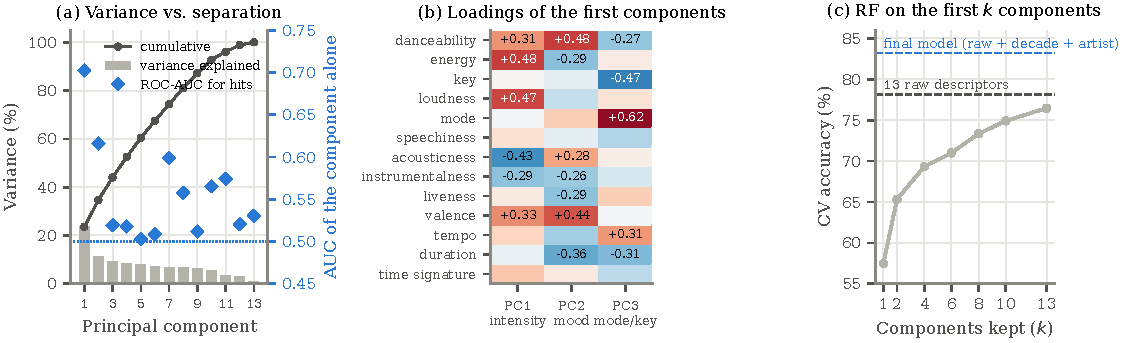
\includegraphics[width=\textwidth]{fig_pca.pdf}
\caption{PCA of the 13 Spotify descriptors (40{,}560 songs). (a) Variance explained by each component
(bars), cumulative (line), and how well each component alone separates hits from non-hits (ROC-AUC, right
axis; dotted line = chance). (b) Loadings of the first three components (values below 0.25 in absolute
value are not printed). (c) Cross-validated accuracy of the frozen Random Forest trained on the first $k$
components, against the 13 raw descriptors and the final model.}
\label{fig:pca}
\end{figure*}

\textbf{Training on everything at once.} One might simply put every input we built into one model. We did
this on the 35{,}370 songs that have a preview (needed for FFT), with the same frozen Random Forest and
$5{\times}5$ CV (Table~\ref{tab:all}). The full model reaches 0.883, 5.8 points above the final model
(0.825 on these songs). That gain does not come from music. Removing the song title alone takes it down to
0.843 ($-4.0$\pp, $p=3\times10^{-19}$), and the title is an artefact of how the non-hits were collected
(App.~\ref{sec:audit}). The remaining $+1.8$\pp{} over the final model must come, by elimination, from FFT and
the market-trend features, the only other blocks that matter (removing either one costs $-0.4$ and $-0.3$\pp; title
length and \texttt{chorus\_hit}/\texttt{sections} change nothing; the two overlap, so each costs less alone), whose gains vanish under the genre control and carry
only the era (App.~\ref{sec:further} and Sec.~\ref{sec:timeseries}). Once FFT and trend are in, the decade
indicators become redundant ($-0.2$\pp, $p=0.11$): all three describe the era. Artist history remains the
input whose removal costs the most among the legitimate ones ($-1.9$\pp, $p=2\times10^{-11}$), ahead of
the 13 descriptors ($-1.2$\pp), while \texttt{chorus\_hit}/\texttt{sections} and title length change nothing.
Training on everything therefore gives a higher number on this benchmark by learning how it was built. The
model we keep is the one whose inputs survive the controls: the 20 inputs of the final model.

\begin{table}[!htbp]
\centering
\caption{Training on every input at once (35{,}370 songs with a preview, frozen Random Forest, $5{\times}5$
CV). Left: one block removed from ``everything'' ($\Delta$ vs everything). Right: the block alone.
$^{*}$Decade alone scores .532 here, not the .503 of the full benchmark, because these songs are 53.2\,\% hits: the
decade carries no information and the model predicts the majority class.}
\label{tab:all}
\footnotesize
\setlength{\tabcolsep}{3pt}
\begin{adjustbox}{max width=\columnwidth}
\begin{tabular}{@{}lccc@{}}
\toprule
Model & Acc. & AUC & $\Delta$ ($p$) \\
\midrule
Final model (Spotify + decade + artist) & .825 & .911 & -- \\
Everything (8 blocks) & \textbf{.883} & .952 & +5.8 ($3{\cdot}10^{-21}$) vs final \\
Everything except song title & .843 & .925 & +1.8 ($6{\cdot}10^{-10}$) vs final \\
\midrule
\multicolumn{4}{@{}l}{\emph{Remove one block from everything}} \\
\quad $-$ song title & .843 & .925 & $-4.0$ ($3{\cdot}10^{-19}$) \\
\quad $-$ artist history & .864 & .933 & $-1.9$ ($2{\cdot}10^{-11}$) \\
\quad $-$ Spotify (13) & .871 & .944 & $-1.2$ ($5{\cdot}10^{-8}$) \\
\quad $-$ FFT (31) & .879 & .949 & $-0.4$ (.01) \\
\quad $-$ market trend (2) & .879 & .949 & $-0.3$ (.01) \\
\quad $-$ decade (6) & .881 & .950 & $-0.2$ (.11) \\
\quad $-$ title length & .883 & .951 & $-0.0$ (.93) \\
\quad $-$ chorus\_hit + sections & .883 & .952 & $+0.0$ (.75) \\
\midrule
\multicolumn{4}{@{}l}{\emph{One block alone}} \\
\quad Spotify (13) / FFT (31) & .777 / .773 & .849 / .847 & -- \\
\quad artist history / song title & .648 / .660 & .669 / .740 & -- \\
\quad market trend / title length & .629 / .546 & .672 / .545 & -- \\
\quad chorus\_hit + sections / decade & .543 / .532$^{*}$ & .563 / .516 & -- \\
\bottomrule
\end{tabular}
\end{adjustbox}
\end{table}

\FloatBarrier
\section{Head-to-head with Du: table}\label{app:tilburg}
\begin{table}[!htbp]
\centering
\caption{Head-to-head with Du~\cite{du2022spotify} using their protocol (one model per
decade, 13 audio + \texttt{chorus\_hit} + \texttt{sections}, 70/30 split) over 50 random
splits: mean accuracy (std). RF: Random Forest; LR: logistic regression; cfg.: configuration. ``Wins'' counts
splits where adding artist history helps; $p$: corrected $t$-test over the $J=50$ paired splits,
$n_{\text{test}}/n_{\text{train}}=3/7$.}
\label{tab:tilburg}
\footnotesize
\setlength{\tabcolsep}{2.6pt}
\begin{adjustbox}{max width=\columnwidth}
\begin{tabular}{@{}llcccc@{}}
\toprule
Dec. & Model & Published & Re-impl. & + artist & Wins / $p$ \\
\midrule
\multirow{3}{*}{00s} & RF (their cfg.) & .84 & .846 (.009) & \textbf{.867} (.009) & 50 / $9{\cdot}10^{-8}$ \\
& LR (their cfg.) & .82 & .821 (.007) & \textbf{.848} (.007) & 50 / $2{\cdot}10^{-9}$ \\
& RF (frozen) & -- & .852 (.008) & \textbf{.875} (.006) & 50 / $10^{-7}$ \\
\midrule
\multirow{3}{*}{10s} & RF (their cfg.) & .82 & .829 (.008) & \textbf{.861} (.008) & 50 / $4{\cdot}10^{-11}$ \\
& LR (their cfg.) & .79 & .807 (.009) & \textbf{.835} (.008) & 50 / $6{\cdot}10^{-6}$ \\
& RF (frozen) & -- & .841 (.008) & \textbf{.873} (.008) & 50 / $9{\cdot}10^{-10}$ \\
\bottomrule
\end{tabular}
\end{adjustbox}
\end{table}

\FloatBarrier
\section{External validation: more detail}\label{app:external}

\begin{figure}[!htbp]
\centering
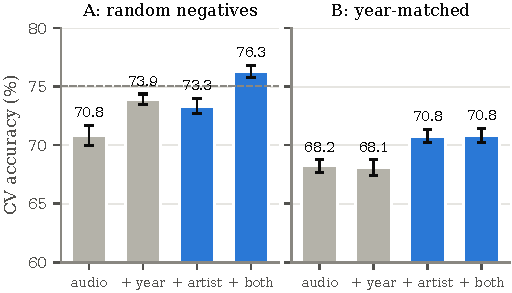
\includegraphics[width=\columnwidth]{fig_ismir.pdf}
\caption{ISMIR 2019 data, cross-validated accuracy with 95\,\% CI. Gray: without artist
history; blue: with it (``both'' = year + artist). Dashed line in A: best published
accuracy~\cite{zangerle2019hit}. Matching years (B) removes the gain of release year but not
that of artist history.}
\label{fig:ismir}
\end{figure}

\begin{table}[!htbp]
\centering
\caption{SpotGenTrack (101{,}909 tracks, 19.4\,\% hits; always predicting ``non-hit''
scores 0.806). 5-fold CV, corrected $t$-test vs the 13 descriptors.}
\label{tab:sgt}
\footnotesize
\setlength{\tabcolsep}{3pt}
\begin{adjustbox}{max width=\columnwidth}
\begin{tabular}{@{}lccc@{}}
\toprule
Features & Acc. [95\,\% CI] & ROC-AUC & $p$ (acc.) \\
\midrule
Spotify descriptors (13) & .812 [.811,.813] & .690 & -- \\
+ decade & .812 [.811,.813] & .712 & .66 \\
+ artist & .823 [.821,.826] & .762 & $10^{-3}$ \\
\textbf{+ decade + artist} & \textbf{.825} [.823,.827] & \textbf{.777} & $3{\cdot}10^{-4}$ \\
+ artist + low-level audio & .825 [.823,.828] & .758 & $2{\cdot}10^{-4}$ \\
\bottomrule
\end{tabular}
\end{adjustbox}
\end{table}

\textbf{SpotGenTrack.} Here the label is Spotify popularity rather than a chart, and
80.6\,\% of tracks are negatives, so accuracy is dominated by the majority class: the 13
descriptors score 0.812, barely above always predicting ``non-hit''. Ranking quality tells
the real story (Table~\ref{tab:sgt}): artist history raises ROC-AUC from 0.690 to 0.762
($+7.2$ points), and with decade to 0.777. On the hit class, the 13 descriptors find
only 8.3\,\% of the hits (F1 0.147); with decade and artist history, recall rises to
25.2\,\% at unchanged precision (0.62) and F1 to 0.358 (5/5 folds, $p=7\times10^{-7}$),
while the 207 low-level audio features add
nothing on top of artist history. A single 75/25 split gives the same picture (accuracy
0.810 $\to$ 0.822 and ROC-AUC 0.688 $\to$ 0.760 with artist history, McNemar
$p=6\times10^{-13}$).


\FloatBarrier
\section{Unseen artists and cold start: table}\label{app:robust}
\begin{table}[!htbp]
\centering
\caption{Robustness. Top: cross-validated accuracy with random stratified folds vs folds
grouped by artist (no test artist seen in training). Era = decade (Hit Predictor) or
release year (ISMIR). Bottom: gain over audio in grouped CV, on songs whose artist had no
earlier hit (new) or at least one (known). New/known songs: 33{,}438/7{,}122 (Hit
Predictor), 7{,}480/4{,}182 (ISMIR A), 7{,}269/4{,}393 (ISMIR B). The accuracy on each group is computed inside
each test fold; the corrected $t$-test uses the per-fold differences on that group and the ratio
$n_{\text{test}}/n_{\text{train}}$ of the whole fold.}
\label{tab:robust}
\footnotesize
\setlength{\tabcolsep}{2.6pt}
\begin{adjustbox}{max width=\columnwidth}
\begin{tabular}{@{}llcccc@{}}
\toprule
Data & Folds & Audio & + era & + artist & + both \\
\midrule
\multirow{2}{*}{Hit Predictor} & random & .782 & .802 & .810 & .832 \\
 & by artist & .772 & .792 & .802 & \textbf{.822} \\
\multirow{2}{*}{ISMIR A} & random & .708 & .739 & .733 & .763 \\
 & by artist & .709 & .739 & .730 & \textbf{.759} \\
\multirow{2}{*}{ISMIR B} & random & .682 & .681 & .708 & .708 \\
 & by artist & .677 & .678 & \textbf{.705} & \textbf{.705} \\
\midrule
& Hits (\%) & \multicolumn{2}{c}{New artists: $\Delta$ ($p$)} & \multicolumn{2}{c}{Known: $\Delta$ ($p$)} \\
\cmidrule(lr){3-4}\cmidrule(l){5-6}
& new/known & + era & + artist & \multicolumn{2}{c}{+ artist} \\
\midrule
Hit Predictor & 39 / 97 & +2.2 ($2{\cdot}10^{-9}$) & +0.4 (.17) & \multicolumn{2}{c}{+15.0 ($3{\cdot}10^{-14}$)} \\
ISMIR A & 36 / 75 & +3.4 ($6{\cdot}10^{-5}$) & +0.8 (.08) & \multicolumn{2}{c}{+4.4 (.003)} \\
ISMIR B & 37 / 72 & +0.1 (.79) & +1.4 (.002) & \multicolumn{2}{c}{+5.3 ($8{\cdot}10^{-5}$)} \\
\bottomrule
\end{tabular}
\end{adjustbox}
\end{table}

\textbf{Artist-grouped cross-validation.} With random folds, songs by the same artist can
fall in both the training and the test part, so a model could recognise an artist from the
audio. We therefore repeat every protocol with stratified group $k$-fold, grouping songs by
normalised artist so that no test artist is seen in training (Table~\ref{tab:robust}, top).
Accuracies drop by up to one point, a small artist-identity effect in the audio
descriptors, but the gains remain: $+5.0$\pp{} for decade and artist on the Hit
Predictor (unchanged, 25/25 folds, $p=10^{-13}$) and $+2.9$\pp{} for artist history in the
year-matched ISMIR protocol (10/10, $p=9\times10^{-7}$). In protocol A the gains lose at
most half a point, and audio, year and artist still reach 0.759 [0.752, 0.766], above the
published 75.04\,\%.

\textbf{Cold start.} Table~\ref{tab:robust} (bottom) splits the grouped test folds by
whether the artist had an earlier hit. On the Hit Predictor, artist history does not help
new artists ($+0.4$\pp, $p=0.17$): its whole gain comes from the 17.6\,\% of songs by
established artists, 96.6\,\% of which are hits, which quantifies the benchmark effect
discussed in Sec.~\ref{sec:discussion}. The decade, in contrast, helps new artists
($+2.2$\pp, $p=2\times10^{-9}$). On ISMIR, where songs by established artists are hits
only 72--75\,\% of the time, artist history also tends to help new artists in the year-matched
protocol ($+1.4$\pp, $p=0.002$, 10/10 folds; above the Bonferroni threshold, so indicative only), perhaps
because an empty history is itself informative when negatives are not selected by artist. On ISMIR, ``new''
means no earlier hit among the dataset's own hits (the reference set there), not in the whole Hot~100.


\FloatBarrier
\section{Audit and further experiments}\label{app:audit}\label{sec:audit}\label{sec:further}
\begin{table}[!htbp]
\centering
\caption{Audit of candidate gains. Single split (McNemar) vs $5{\times}5$ cross-validation
(corrected $t$-test). Top: full benchmark (single split = the canonical split, 2{,}000 test songs). Bottom:
3{,}562-song audio subset (single split = its stratified 75/25 split, 891 test songs).}
\label{tab:audit}
\footnotesize
\setlength{\tabcolsep}{2.6pt}
\begin{adjustbox}{max width=\columnwidth}
\begin{tabular}{@{}lcccl@{}}
\toprule
Added to audio & Split $\Delta$ ($p$) & CV $\Delta$ & CV $p$ & Verdict \\
\midrule
Song title (TF-IDF) & +6.9 ($4{\cdot}10^{-14}$) & +6.7 & $4{\cdot}10^{-20}$ & artefact \\
\texttt{chorus\_hit}+\texttt{sections} & +0.6 (.32) & $-$0.0 & .82 & no effect \\
Title length & +0.05 (1.0) & +0.2 & .28 & no effect \\
\midrule
Rich librosa (PCA 40) & +3.8 (.002) & +0.9 & .15 & not significant \\
FFT descriptors (31) & +4.4 (.001) & +2.3 & .007 & small \\
Decade & +1.1 (.27) & +1.0 & .03 & small \\
Artist & +3.4 (.010) & +3.8 & $2{\cdot}10^{-6}$ & robust \\
Artist + rich & +6.7 ($10^{-6}$) & +4.9 & $10^{-8}$ & = artist \\
Decade + artist & +3.6 (.006) & +5.1 & $10^{-8}$ & robust \\
\bottomrule
\end{tabular}
\end{adjustbox}
\end{table}

\textbf{Titles.} A title model trained out-of-fold adds $+6.7$\pp, more than any musical
feature. Its largest weights show why. On the non-hit side: \emph{remastered, feat, live, version, remix, mix,
edit, demo, mono, medley}, genre words (\emph{blues, metal, ambient, punk, rock, death, jazz, hardcore}) and
non-English words (\emph{remasterizado, de, te, en}); on the hit side: ordinary words (\emph{nights, you, party,
kiss, love, sunshine}). On the genre-matched sample of App.~\ref{sec:further} (7{,}554 songs), 13.5\,\% of the
non-hit titles contain `` - '' (a Spotify suffix such as ``- Remastered 2011''), against 0.1\,\% of the hits;
5.7\,\% contain ``remaster'' (hits: 0), and 5.7\,\% contain non-ASCII letters (hits: 0.1\,\%). The hit titles have
evidently been cleaned and the non-hit titles have not. We test this directly (\texttt{r8\_future\_work.py title},
$5{\times}5$ CV on the genre-matched sample). The title adds $+4.8$\pp{} to the 13 descriptors and $+2.9$\pp{} to
the final model (25/25, $p=2\times10^{-6}$), so genre explains only part of it. We then strip everything after
`` - '', anything in brackets and ``feat./ft./featuring \dots'' (this changes 19.0\,\% of non-hit titles and 4.9\,\%
of hit titles). The gain over the final model falls to $+1.9$\pp{} (23/25, $p=0.002$), above the Bonferroni
threshold. What remains is mostly genre and language vocabulary. We reject the title: its gain comes from how the
two classes were written down and collected, not from anything that makes a song a hit.

\textbf{Single split vs cross-validation.} On the small audio subset, the 185 rich librosa
descriptors appeared to add $+3.8$\pp{} with $p=0.002$ on the subset's single 75/25 split, but the
cross-validated gain is $+0.9$\pp{} and is not significant. The same holds for the choice
of the PCA dimension (5 to 100 components are within noise) and for the knock-out of any
descriptor family (all within $\pm0.1$\pp). In a block ablation of the full subset model,
only removing artist history causes a significant drop ($-3.3$\pp, $p=10^{-5}$). The
\texttt{chorus\_hit} and \texttt{sections} fields, often suspected of leakage, add nothing.

\textbf{FFT and the best audio-subset model.} The 31 FFT descriptors are the only extra
audio representation whose gain survives cross-validation, and it persists on top of
artist history: audio + artist + FFT reaches $0.821$ against $0.801$ for audio + artist
($+2.0$\pp, 23/25 folds, $p=0.008$). Adding decade to that model gives the best subset
accuracy, $0.824$, but the increment is not significant ($+0.3$\pp, $p=0.50$), and
decade adds nothing to FFT alone ($0.785$ with decade vs $0.786$ without): the spectral descriptors already
carry the era. Conversely, artist history still adds $+3.5$\pp{} on top of FFT
($p=4\times10^{-5}$). Fig.~\ref{fig:subset} shows every configuration we evaluated on
this subset.

\textbf{FFT on the whole benchmark.} We then retrieved Deezer previews for every song we
could match: 35{,}370 of the 40{,}560 songs (87.2\,\%). Deezer finds hits more often than
flops (94.0\,\% vs 80.6\,\%), so the covered set is 53.2\,\% hits and every comparison
below uses the same 35{,}370 songs. With $5{\times}5$ cross-validation, adding FFT to the
main model (audio + decade + artist) raises accuracy from $0.825$ to $0.839$ ($+1.4$\pp,
25/25 folds, $p=4\times10^{-9}$; AUC $0.911\to0.921$). The whole gain comes from songs by
new artists, $0.789\to0.807$ ($+1.8$\pp, 25/25, $p=6\times10^{-9}$), while songs by known
artists stay at $0.977$ ($-0.1$\pp, n.s.). Unlike on the small subset, decade remains
useful once FFT is present: audio + artist + FFT reaches only $0.829$ ($+0.4$\pp{} over the
main model, $p=0.04$). FFT thus appears to address the cold-start weakness of artist
history, but the benchmark's flops come from non-mainstream genres by construction, and
spectral descriptors can recognise genre. App.~\ref{sec:further} shows that this gain does
not survive a genre control.

\begin{figure}[!htbp]
\centering
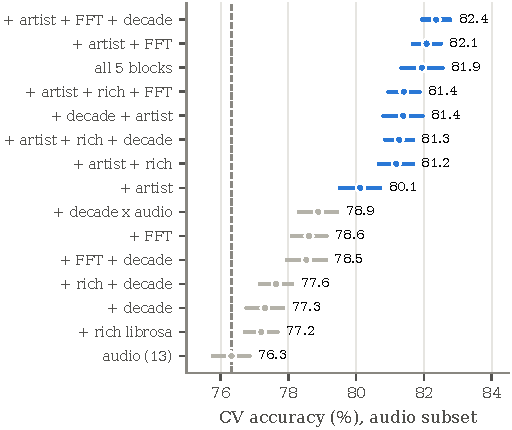
\includegraphics[width=\columnwidth]{fig_subset.pdf}
\caption{Every configuration evaluated on the 3{,}562-song audio subset, $5{\times}5$
cross-validated accuracy with 95\,\% CI, sorted. Blue: with artist history; gray: without.
Dashed line: the 13 Spotify descriptors alone. ``rich'': the 185 librosa descriptors (PCA 40); ``decade x
audio'': each of the 13 descriptors multiplied by each of the 6 decade indicators (78 inputs); ``all 5 blocks'':
audio + artist + decade + decade x audio + rich.}
\label{fig:subset}
\end{figure}


\textbf{Genre control for FFT.} We attach Spotify artist genres from the SpotGenTrack
release~\cite{martingutierrez2020multimodal} by normalised artist name (20{,}610 songs
with both a preview and a genre) and map the tags to 16 families. The benchmark's
construction is plainly visible: Latin, classical, jazz, ``world'' and metal artists
account for 50\,\% of the flops and 1.9\,\% of the hits, while rock, pop, R\&B,
hip-hop and country account for 93\,\% of the hits. Genre is also partly audible: a
Random Forest (200 trees, stratified shuffled 5-fold cross-validated predictions, seed 42) recovers the dominant
family from the 13 Spotify descriptors with 47.4\,\% accuracy,
from the 31 FFT descriptors with 49.9\,\% and from both with 53.3\,\% (majority class
26.1\,\%). Three results follow (Table~\ref{tab:genre}). (a) Genre families as features
raise the main model from $0.828$ to $0.928$ ($+10.1$\pp, 25/25, $p=8\times10^{-23}$):
on this benchmark, knowing the artist's genre is worth more than any audio
representation. (b) Once genre is known, FFT \emph{lowers} accuracy ($-1.1$\pp, 0/25,
$p=5\times10^{-7}$), also for new artists ($-1.4$\pp). (c) On a genre-matched sample
(as many hits as flops inside every family; 7{,}554 songs), FFT adds nothing to the main
model ($+0.1$\pp, 13/25, $p=0.84$; new artists $+0.1$\pp, $p=0.80$). FFT still improves
the 13 Spotify descriptors alone on that sample ($+2.5$\pp, 25/25, $p=5\times10^{-4}$),
but the main model, without FFT, still beats audio + FFT by $4.3$\pp{}
($p=2\times10^{-8}$), and decade and artist history add $+6.7$\pp{} to the 13 descriptors on that sample
(0.722 $\to$ 0.790, 25/25, $p=9\times10^{-13}$); each one alone also helps on that sample (decade $+2.5$\pp,
$p=8\times10^{-7}$; artist history $+4.2$\pp, $p=2\times10^{-8}$; \texttt{r8\_future\_work.py decadegenre}). We conclude that the full-benchmark FFT gain is a genre shortcut,
whereas the gain of artist history survives the genre control. Spotify assigns artist
genres retrospectively, so we use them only as a control, never as a predictive feature.

\begin{table}[!htbp]
\centering
\caption{Genre control for FFT ($5{\times}5$ CV). Left: songs with a preview and a Spotify
genre. Right: genre-matched sample. Accuracy overall and on songs by new artists.}
\label{tab:genre}
\setlength{\tabcolsep}{3pt}
\begin{tabular}{lcccc}
\toprule
& \multicolumn{2}{c}{All (20{,}610)} & \multicolumn{2}{c}{Matched (7{,}554)} \\
Model & Acc. & new art. & Acc. & new art. \\
\midrule
audio (13 descriptors) & -- & -- & .722 & -- \\
main (audio+decade+artist) & .828 & .780 & .790 & .749 \\
\quad + FFT & .841 & .798 & .791 & .750 \\
\quad + genre & .928 & .911 & -- & -- \\
\quad + genre + FFT & .917 & .897 & -- & -- \\
\midrule
decade vs audio, $\Delta$ ($p$) & \multicolumn{2}{c}{--} & \multicolumn{2}{c}{$+2.5$ ($8{\cdot}10^{-7}$)} \\
artist vs audio, $\Delta$ ($p$) & \multicolumn{2}{c}{--} & \multicolumn{2}{c}{$+4.2$ ($2{\cdot}10^{-8}$)} \\
main vs audio, $\Delta$ ($p$) & \multicolumn{2}{c}{--} & \multicolumn{2}{c}{$+6.7$ ($9{\cdot}10^{-13}$)} \\
FFT vs main, $\Delta$ ($p$) & \multicolumn{2}{c}{$+1.3$ ($1.1{\cdot}10^{-4}$)} & \multicolumn{2}{c}{$+0.1$ (.84)} \\
FFT vs main+genre, $\Delta$ ($p$) & \multicolumn{2}{c}{$-1.1$ ($5{\cdot}10^{-7}$)} & \multicolumn{2}{c}{--} \\
\bottomrule
\end{tabular}
\end{table}

\textbf{Artist resolution.} The 52.1\,\% match rate is not a matching problem: 99.99\,\%
of the hits have an artist found in the chart history (by construction, at the latest in their own decade),
against 5.4\,\% of the flops, and only 2.7\,\% of the flops have an artist who charted up to and including their
own decade (only about 1.2\,\% charted in an \emph{earlier} decade, i.e.\ have $h(s)>0$). The remaining
$\approx$1.5\,\% of flops have an artist whose normalised name has a Hot~100 entry in the flop's own decade,
although the dataset's rule excludes such artists: these are homonyms merged by our name matching, or chart
entries missing from the dataset's own hit list; they do not enter $h(s)$, which counts earlier decades only.
The unmatched songs are flops whose artists never charted. Two alternatives give
no gain: matching the full credited name before the primary artist (``Simon \&
Garfunkel'' rather than ``Simon'') lowers accuracy ($0.827$ vs $0.832$, $-0.5$\pp,
$p=4\times10^{-4}$), and crediting featured appearances changes nothing ($+0.1$\pp,
$p=0.39$). Canonical identifiers would avoid homonyms but cannot raise the match rate.

\textbf{How fast does a model age?} We train on a single decade and test on every later
one (Table~\ref{tab:decay}, songs with a preview). Audio-only accuracy falls from
$0.809$ within a decade to $0.765$ one decade later and $0.689$ three decades later.
Artist history slows the decay, and its advantage grows with the gap ($+2.8$\pp{} within
a decade, $+5.1$\pp{} three decades later). FFT behaves in the opposite way: it helps
within a decade ($+2.2$\pp) but hurts from three decades on, consistent with descriptors
that encode era-specific production and genre rather than lasting appeal. The cells
average 6 to 1 train/test pairs and are not tested for significance.

\begin{table}[!htbp]
\centering
\caption{Model ageing: train on one decade, test $k$ decades later (frozen Random Forest of the main model, one fit
per pair,
35{,}370 songs with a preview; $k=0$: 5-fold CV inside each decade). Mean accuracy over
the available decade pairs.}
\label{tab:decay}
\setlength{\tabcolsep}{4pt}
\begin{tabular}{cccccc}
\toprule
$k$ & pairs & audio & + artist & + FFT & + artist + FFT \\
\midrule
0 & 6 & .809 & .837 & .831 & \textbf{.859} \\
1 & 5 & .765 & .796 & .782 & \textbf{.810} \\
2 & 4 & .728 & \textbf{.775} & .736 & \textbf{.775} \\
3 & 3 & .689 & \textbf{.740} & .673 & .728 \\
4 & 2 & .666 & \textbf{.734} & .661 & .718 \\
5 & 1 & .664 & \textbf{.754} & .599 & .706 \\
\bottomrule
\end{tabular}
\end{table}

\textbf{Lyrics on SpotGenTrack.} SpotGenTrack provides six lexical descriptors of the lyrics (syllables
per word, words per sentence, sentence count, word count, sentence similarity,
vocabulary richness) for 79{,}420 tracks with lyrics (21.5\,\% hits; $5{\times}1$ CV as in
Sec.~\ref{sec:external}). They improve the 13 Spotify descriptors (AUC $0.678\to0.729$,
$p=3\times10^{-4}$) and still add on top of decade and artist history (accuracy
$0.808\to0.814$, 5/5 folds, $p=0.002$; AUC $0.774\to0.797$, $p=2\times10^{-5}$). The gain
is modest in accuracy because of the class imbalance, and such a small gain measured on five folds does not
survive the Bonferroni correction, so we tested lyrics again on a larger, balanced dataset.


\FloatBarrier
\section{Lyrics on ISMIR: more detail}\label{app:lyrics}
ISMIR songs are Million Song Dataset tracks (joined to the lyrics by their MSD track identifier), for which the official musiXmatch
release~\cite{bertinmahieux2011million} gives the lyrics of 237{,}662 tracks as word counts over the
5{,}000 most frequent (stemmed) words. Coverage is itself a shortcut: 56\,\% of the hits have lyrics against
36\,\% of the non-hit pool, so ``has lyrics'' would predict the label. We therefore keep only songs
\emph{with} lyrics on both sides and redraw balanced samples under protocols A and B. A second shortcut is
language: 97.5\,\% of the hits but only 80.5\,\% of the non-hits are mainly in English (at least 25\,\% of
their words among the 29 most common English words). We therefore also repeat every test on English songs
only: the non-English songs are removed first, and the balanced (protocol A) or year-matched (protocol B) sample is
then drawn again from what remains. Two lyrics inputs are added to the final ISMIR model (audio + year + artist history): eight lexical
features (log number of words and of distinct words, richness, repetition, share of \emph{I/me/my},
\emph{you/your}, \emph{love} and of common English words), and one bag-of-words score, the out-of-fold
probability of a TF-IDF logistic regression trained inside each training fold, as for titles.

\begin{table}[!htbp]
\centering
\caption{Lyrics on ISMIR 2019 (songs with lyrics only; Random Forest, $5{\times}2$ CV, corrected $t$-test
vs the final model of the same row; all rows 10/10 folds improved). Unseen: no artist in both training and
test folds.}
\label{tab:lyrics}
\footnotesize
\setlength{\tabcolsep}{2.6pt}
\begin{adjustbox}{max width=\columnwidth}
\begin{tabular}{@{}lccccc@{}}
\toprule
Sample & Songs & Final & + lyrics & $\Delta$ ($p$) & AUC \\
\midrule
A: random & 6{,}526 & .728 & \textbf{.775} & +4.7 ($3{\cdot}10^{-4}$) & .798$\to$.851 \\
B: year-matched & 6{,}478 & .676 & \textbf{.727} & +5.1 ($2{\cdot}10^{-5}$) & .732$\to$.802 \\
A, English & 6{,}364 & .718 & \textbf{.745} & +2.7 ($6{\cdot}10^{-4}$) & .788$\to$.820 \\
B, English & 6{,}294 & .658 & \textbf{.708} & +4.9 ($1.1{\cdot}10^{-4}$) & .720$\to$.772 \\
A, English, unseen & 6{,}364 & .712 & \textbf{.742} & +3.0 ($6{\cdot}10^{-4}$) & .785$\to$.817 \\
B, English, unseen & 6{,}294 & .656 & \textbf{.700} & +4.4 ($3{\cdot}10^{-5}$) & .717$\to$.764 \\
\midrule
\multicolumn{6}{@{}l}{Lyrics alone (the 8 lexical features + bag-of-words score, no audio, year or artist; B, year-matched): .702,} \\
\multicolumn{6}{@{}l}{above the final model without lyrics (.676). Artist history uses all ISMIR hits as reference set.} \\
\bottomrule
\end{tabular}
\end{adjustbox}
\end{table}

Table~\ref{tab:lyrics} and Fig.~\ref{fig:lyrics}a show that lyrics add $+4.7$ points in protocol~A and
$+5.1$ in the year-matched protocol~B, in all 10 folds. The gain shrinks but remains when only English songs are
kept ($+2.7$ and $+4.9$), and it remains when, in addition, no artist appears in both training and test folds
($+3.0$ and $+4.4$, $p=3\times10^{-5}$; AUC $+0.047$, $p=10^{-6}$), so it does not come from recognising the
vocabulary of artists seen in training. In the strictest setting (year-matched, English, unseen artists) the gain
survives the Bonferroni correction ($p=3\times10^{-5}<1.25\times10^{-4}$), as do the other protocol-B rows; the
three protocol-A rows ($p=3\times10^{-4}$ to $6\times10^{-4}$) do not, and are indicative only. In the year-matched
protocol, lyrics alone (0.702) are more accurate than audio, year and artist history together (0.676).
Fig.~\ref{fig:lyrics}b shows what the model reads. Hit lyrics favour \emph{love} (by far the largest weight),
vocables (\emph{la}, \emph{oh}, \emph{ooh}, \emph{yeah}, \emph{hey}) and direct address (\emph{need},
\emph{girl}) and night-out themes (\emph{night}). Non-hit lyrics favour darker or narrative words (\emph{kill}, \emph{hate},
\emph{crime}, \emph{mind}, \emph{their}, \emph{the}). On average, hit lyrics are slightly longer and use a
smaller share of distinct words (richness 0.34 vs 0.42), use \emph{love} twice as often (1.3\,\% vs 0.65\,\% of words) and
use \emph{you} more (5.5\,\% vs 4.6\,\%). These words point to themes and genres (romantic pop against metal,
punk or hardcore rap) as much as to style. On ISMIR this is a real difference between chart songs and the rest of
the catalogue rather than a construction rule, since the negatives are drawn at random. But it means that lyrics,
like genre, tell \emph{mainstream} songs from the rest more than they measure the appeal of an individual song.
We could not test lyrics on the Hit Predictor, whose songs have no Million Song Dataset identifier.


\FloatBarrier
\section{Time series: chart components, market trend, trajectory table}\label{app:tsdetails}
\textbf{The chart as a time series.} The weekly Hot~100 (3{,}545 charts, 1958--2026) also
forms time series. A \emph{debut} is the first week a (title, performer) pair appears anywhere in the chart
history (re-entries are not debuts). The monthly mean number of debuts per chart week (1959--2025) is mostly
trend: an STL decomposition~\cite{cleveland1990stl} gives a trend strength of 0.72 and a
seasonal strength of 0.11~\cite{hyndman2021forecasting}. Debuts fall from 11.0 per week in
1959 to 5.5 in 2001 and return to 10.9 in 2025, after the chart started counting streams;
the largest residual is a rule change (60 debuts in the chart of 5 December 1998, when
songs not released as singles became eligible). The weekly number of holiday songs on the
chart is almost purely seasonal: its periodogram peaks at 52.1, 26.1, 17.4 and 13.0 weeks,
and a Fourier regression fitted on the streaming era (charts from July 2018 on, a recent window in which streaming dominates the chart; target $\ln(1+\text{count})$, a linear trend plus $K=20$ harmonics) explains 94\,\% of
its variance. Forecasting monthly debuts 12 months ahead under rolling-origin evaluation
(11 origins, 2015--2025), ARIMA$(1,1,2)$~\cite{box2015time} and ARIMA with Fourier terms
(MASE 1.82) and damped Holt-Winters (1.85) are best and indistinguishable (ARIMA + Fourier vs ARIMA, $p=0.97$); they
beat the seasonal naive forecast (2.32) at 10 of 11 origins ($p=0.006$). Both $p$-values come from a two-sided
paired $t$-test on the 11 per-origin MASE values (the 12-month test windows of different origins do not overlap). A seasonal ARIMA
(1.89) and gradient boosting or random forests on lag and Fourier features (1.94, 1.99) do
worse: the series has little seasonality, and 800 points leave tree models little to learn.

\textbf{Before release: market trends.} We describe each Hit Predictor song by the
distance of its standardised audio descriptors to the centroid of the previous decade's
hits, and by its projection on the direction in which that centroid moved. On top of the
main model these two features add $+0.07$\pp{} ($p=0.66$); the 13 per-feature deviations add
$+0.46$\pp{} (23/25, $p=0.006$). On audio alone the trend features add $+1.8$\pp{}
($p=7\times10^{-10}$), less than the decade alone ($+2.0$\pp): they carry era information,
which the main model already has.


\begin{table}[!htbp]
\centering
\caption{Predicting a top-10 peak from a song's first $k$ weeks on the Hot~100 (31{,}925
songs, 16.4\,\% top-10; Random Forest, $5{\times}3$ CV). Values are ROC-AUC except the F1 column (F1 on the
top-10 class of the weeks + context model, threshold 0.5). Context: year, month and the
artist's earlier chart history. Last column: songs not yet in the top~10 after $k$ weeks (ROC-AUC).}
\label{tab:traj}
\setlength{\tabcolsep}{4pt}
\begin{tabular}{ccccc|c}
\toprule
 & \multicolumn{4}{c|}{All songs} & Not yet top 10 \\
$k$ & weeks & + context & F1 & context only & + context \\
\midrule
1 & .700 & .750 & .401 & .593 & .720 \\
2 & .796 & .850 & .531 & .593 & .828 \\
3 & .845 & \textbf{.892} & .610 & .593 & .870 \\
4 & .891 & \textbf{.917} & .674 & .593 & .894 \\
\bottomrule
\end{tabular}
\end{table}


\FloatBarrier
\section{Single splits and multiple comparisons}\label{app:stats}
\textbf{Single splits mislead.} Several conclusions of our own earlier single-split
analysis did not survive cross-validation. With a few thousand songs, an 891-song test set
has a standard error of about 1.4\pp, so single-split gains of 3--4\pp{} on subsets are
fragile even when McNemar's test is significant on that split.
\textbf{Multiple comparisons.} Each $p$-value printed in the paper is the raw value of its own test. Bonferroni
divides 0.05 by the number of tests in the family. We take as family every $p$-value printed in a table or in the
text that compares two configurations, counting a test again each time it is printed (the survival ranking,
Tables~\ref{tab:main}, \ref{tab:models}, \ref{tab:tilburg}, \ref{tab:ismir}, \ref{tab:sgt}, \ref{tab:robust},
\ref{tab:audit}, \ref{tab:all}, \ref{tab:genre}, \ref{tab:lyrics}, the ablation and the values given only in the
text), plus the exploratory tests we ran but do not print one by one: the PCA dimensions of the librosa block, the
knock-out of each librosa descriptor family and the configurations of Fig.~\ref{fig:subset} (on the audio
subset: 7 PCA settings, 8 family knock-outs and 13 configurations, i.e.\ fewer than 30 tests). Rather than rely on an
exact count, we use a deliberately generous family of 400, well above that total; the threshold is
$p<0.05/400=1.25\times10^{-4}$.

Every result our conclusions rest on passes it: the cross-validated gains of Tables~\ref{tab:main}
and~\ref{tab:models} ($p\leq4\times10^{-5}$), the head-to-head of Table~\ref{tab:tilburg} ($\leq6\times10^{-6}$),
the temporal hold-out ($\leq10^{-7}$), the ISMIR gains of artist history in both protocols ($\leq3\times10^{-5}$),
the artist-grouped gains, the genre-matched gains of decade ($8\times10^{-7}$), artist history ($2\times10^{-8}$)
and both ($9\times10^{-13}$), and the year-matched lyrics tests (protocol B: $2\times10^{-5}$; English only:
$1.1\times10^{-4}$; English, unseen artists: $3\times10^{-5}$). The full-benchmark FFT gain on top of the main model
also passes ($p=4\times10^{-9}$) but is explained by genre (App.~\ref{sec:further}); the genre-control results
themselves ($p\leq5\times10^{-7}$) pass as well, and so do the early-trajectory gains of Table~\ref{tab:traj}
($p<10^{-6}$).

Results with $1.25\times10^{-4}\leq p<0.05$ are indicative only: on the 2{,}000-song canonical split, decade alone
($3\times10^{-4}$) and artist history alone ($6\times10^{-4}$); the decade and FFT gains on the 3{,}562-song audio
subset (including FFT on top of artist history) and most single-split gains on that subset; audio + artist + FFT
against the main model on the whole benchmark ($p=0.04$); the per-feature market-trend deviations ($p=0.006$); the
forecasting comparison of Sec.~\ref{sec:timeseries} ($p=0.006$, 11 origins); the lyrics gains on SpotGenTrack
($5{\times}1$ CV, $p=0.002$) and the three protocol-A lyrics rows of ISMIR ($3\times10^{-4}$ to $6\times10^{-4}$); the
SpotGenTrack gains of artist history ($10^{-3}$) and of decade + artist ($3\times10^{-4}$), which are in any case
upper bounds (popularity is measured today, Sec.~\ref{sec:discussion}); the release-year gain on ISMIR A
($2\times10^{-4}$), a shortcut anyway; and the ISMIR cold-start gains of artist history for known artists in
protocol A and new artists in protocol B.


\section{Which script produces what}\label{app:scripts}

\begin{table}[h]
\centering
\caption{Scripts in \texttt{repro/} and the results they produce (\texttt{paper\_results/r*\_*.csv}).}
\label{tab:scripts}
\footnotesize
\setlength{\tabcolsep}{3pt}
\begin{tabular}{@{}l>{\raggedright\arraybackslash}p{3.6cm}@{}}
\toprule
Script & Results \\
\midrule
\texttt{r1\_kaggle\_core.py} & main result, per decade, titles, chorus\_hit (Tables~\ref{tab:main}, \ref{tab:decade}) \\
\texttt{r2\_models\_time.py} & five classifiers, SHAP, future decades (Table~\ref{tab:models}) \\
\texttt{r3\_audio\_subset.py} & audio subset, librosa, FFT (Table~\ref{tab:audit}, Fig.~\ref{fig:subset}) \\
\texttt{r4\_external.py} & ISMIR, SpotGenTrack (Tables~\ref{tab:ismir}, \ref{tab:sgt}) \\
\texttt{r5\_tilburg.py} & head-to-head with Du (Table~\ref{tab:tilburg}) \\
\texttt{r6\_robustness.py} & unseen artists, cold start (Table~\ref{tab:robust}) \\
\texttt{r7\_fft\_full.py} & FFT on the whole benchmark \\
\texttt{r8\_future\_work.py} & artist matching, genre control, decay, SpotGenTrack lyrics (Tables~\ref{tab:genre}, \ref{tab:decay}) \\
\texttt{r9\_metrics.py} & precision, recall, F1 \\
\texttt{r10\_timeseries.py} & market trend, early trajectories (Table~\ref{tab:traj}) \\
\texttt{r11\_lyrics\_ismir.py} & lyrics on ISMIR (Table~\ref{tab:lyrics}, Fig.~\ref{fig:lyrics}) \\
\texttt{r12\_report.py} & PCA, ablation, everything together, trajectory figure (Sec.~\ref{sec:ablation}, Fig.~\ref{fig:traj}) \\
\texttt{r13\_explain.py} & worked example and decade medians (Figs.~\ref{fig:algorithm}, \ref{fig:decade}) \\
\texttt{make\_figures.py} & all data figures \\
\texttt{timeseries/} \texttt{build\_notebook.py} & STL, periodogram, Fourier, ARIMA forecasting (App.~\ref{app:ts}) \\
\bottomrule
\end{tabular}
\end{table}

\section{Time-series details}\label{app:ts}

The chart analysis of Sec.~\ref{sec:timeseries} is in a notebook (\texttt{timeseries/time\_series\_hot100.ipynb})
that follows the standard sequence of a time-series study~\cite{hyndman2021forecasting}: plot the series,
decompose it into trend, seasonality and residual, look for cycles with the periodogram, model the cycles
with Fourier terms, test stationarity (ADF, KPSS) and autocorrelation (ACF, PACF, Ljung--Box), and compare
forecasting methods by rolling origin.

\begin{figure}[h]
\centering
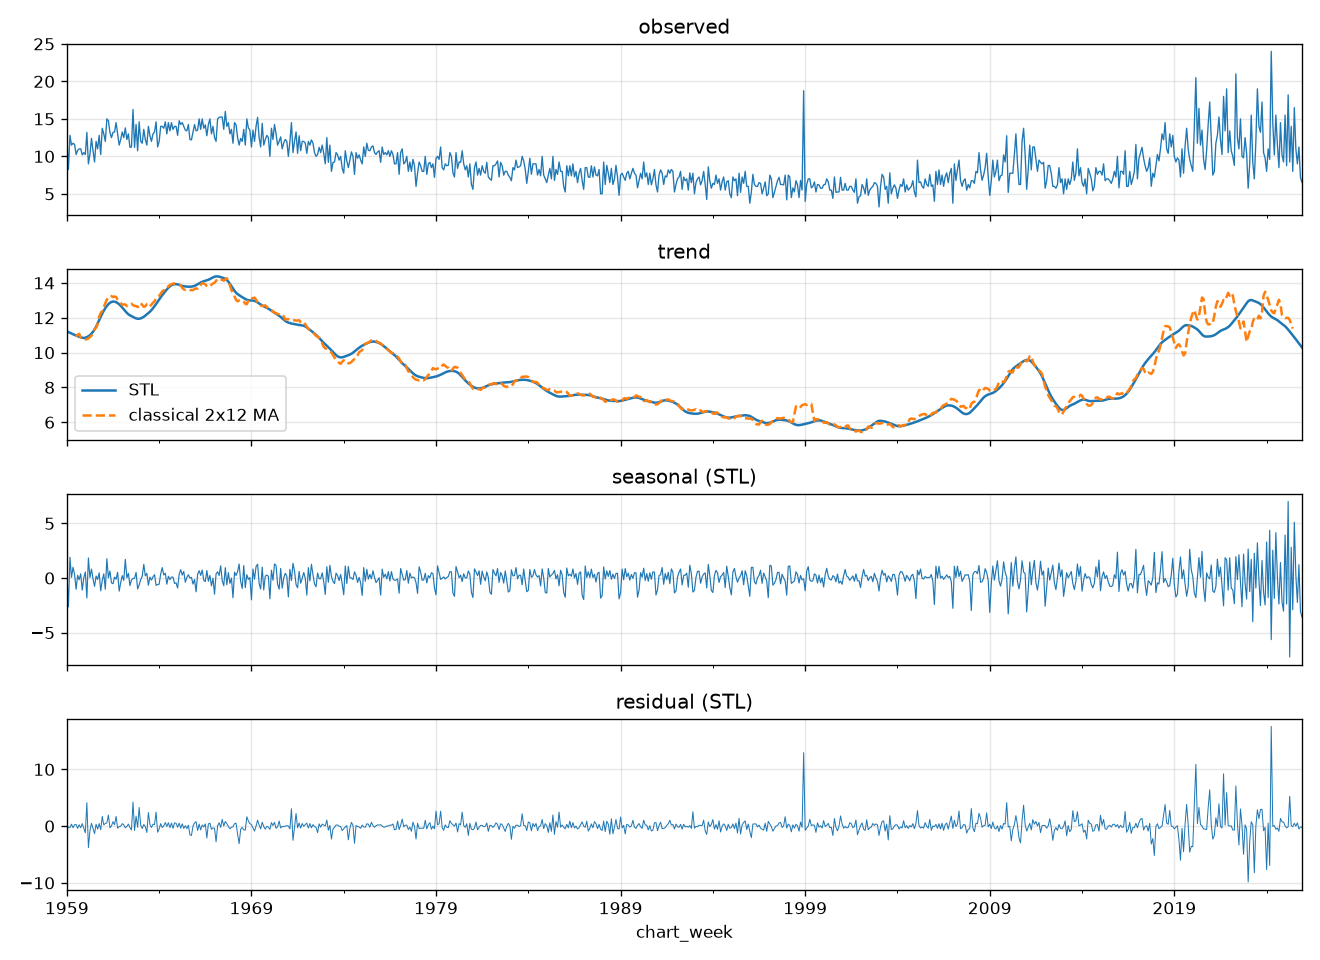
\includegraphics[width=\columnwidth]{ts_decomposition.png}
\caption{STL decomposition of the monthly mean number of debuts per chart week (1959--2025). The trend
dominates (strength 0.72); seasonality is weak (0.11). The spike of December 1998 is the rule change that
admitted songs not released as singles.}
\label{fig:stl}
\end{figure}

\begin{figure}[h]
\centering
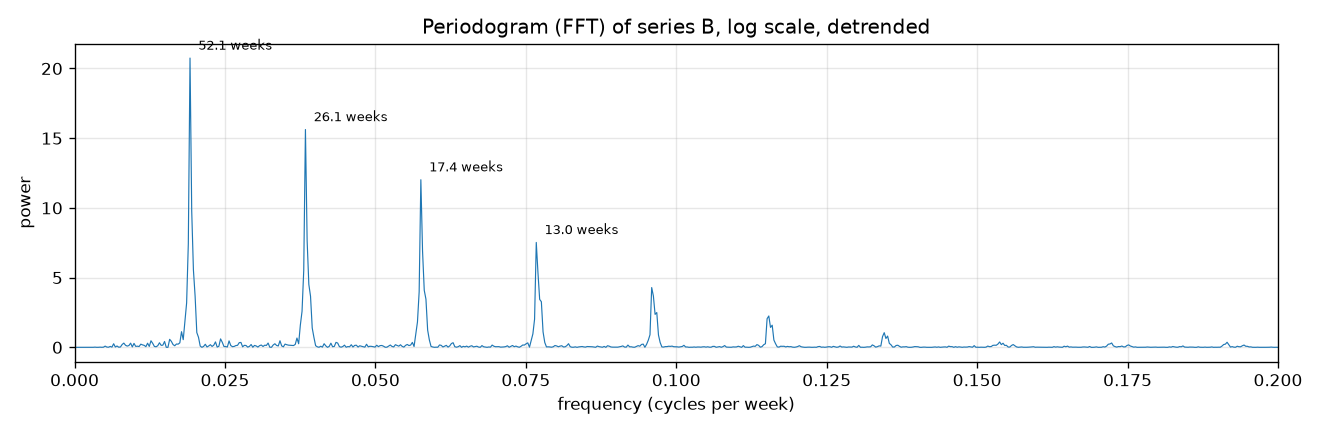
\includegraphics[width=\columnwidth]{ts_periodogram.png}
\caption{Periodogram (FFT) of the weekly number of holiday songs on the chart: peaks at one year and its
harmonics (26.1, 17.4, 13.0 weeks), which a Fourier regression turns into the seasonal pattern.}
\label{fig:periodogram}
\end{figure}

\begin{figure}[h]
\centering
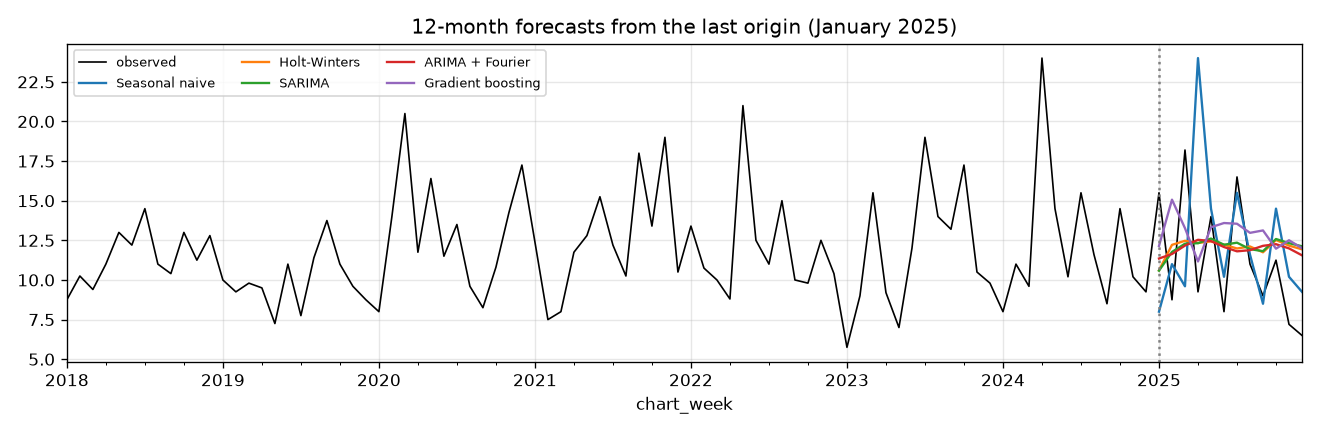
\includegraphics[width=\columnwidth]{ts_forecasts.png}
\caption{Twelve-month forecasts of monthly debuts from the last origin (January 2025).}
\label{fig:forecasts}
\end{figure}

\begin{table}[h]
\centering
\caption{Forecasting monthly debuts 12 months ahead, rolling origin (11 origins, 2015--2025). MASE: mean
absolute error divided by that of the in-sample seasonal naive forecast (lower is better).}
\label{tab:forecast}
\footnotesize
\begin{tabular}{@{}lc@{}}
\toprule
Method & MASE \\
\midrule
ARIMA$(1,1,2)$ & \textbf{1.82} \\
ARIMA$(1,1,2)$ + Fourier terms & \textbf{1.82} \\
Damped Holt--Winters (ETS) & 1.85 \\
Seasonal ARIMA & 1.89 \\
Gradient boosting, lags + Fourier & 1.94 \\
Random forest, lags + Fourier & 1.99 \\
Seasonal naive & 2.32 \\
\bottomrule
\end{tabular}
\end{table}

\textbf{ARIMA in one paragraph.} ARIMA$(p,d,q)$ models a series by differencing it $d$ times until it has
no trend, then explaining each value from its own $p$ previous values (autoregression) and from the $q$
previous forecast errors (moving average). We chose $d=1$ from the stationarity tests and $(p,q)$ by AIC
over $p,q\leq2$. Adding Fourier terms as regressors captures yearly seasonality with few parameters.

\section{Questions a reader may ask}\label{app:faq}

\textbf{Is artist history not cheating?} No information from the song's own period or later is used
(Fig.~\ref{fig:history}), so it is available on release day. What inflates its gain on the Hit Predictor
is the construction of the negatives (artists of hits are excluded), which is why we report the
year-matched ISMIR gain ($+2.6$\pp) as the transferable number.

\textbf{Why does the paper say the gain holds for unseen artists but not for new artists?} The two words
mean different things (Sec.~\ref{sec:features}): an unseen artist is absent from the training folds but may
have earlier hits; a new artist has none, so $h(s)=0$.

\textbf{Why Random Forest and not XGBoost?} XGBoost is 1.3 points better under cross-validation but ties
on the canonical split ($p=0.87$); the frozen Random Forest keeps our numbers comparable with the published
configuration, and the gain of our features is the same for all five classifiers (Table~\ref{tab:models}).

\textbf{Why no deep learning?} The question is which inputs carry signal, at equal model. A learned audio
representation could capture what the descriptors miss, and is future work.

\textbf{Why reject the song title when it is the strongest feature?} A title does not make a song a hit.
It reveals how the non-hits were collected (niche-genre catalogue tracks), so its gain would not transfer
to any other dataset.

\textbf{Why does release year alone score below chance (0.448) in ISMIR protocol~B?} Every hit has a
non-hit from the same year, so the year carries no information, and a Random Forest on a single input with
many distinct values fits noise in the training folds; with exactly balanced years, what it learns for a
year is then, on average, the opposite of the test fold's labels for that year, which pushes it below 0.5.

\textbf{Why is FFT rejected although its gain is significant on the whole benchmark?} Because it vanishes
when hits and non-hits come from the same genres (Table~\ref{tab:genre}): spectral descriptors recognise the
niche genres from which the benchmark draws its non-hits.

\textbf{Why are the canonical numbers lower than the cross-validated ones?} The canonical split trains on
20{,}000 songs, cross-validation on 32{,}448; with more training data every configuration is about one point
better, and the differences between configurations are the same.

\textbf{Why are lyrics kept but not genre, if lyrics also partly reflect genre?} Spotify genre tags
describe the artist as known today, so they are not known on release day.
The words of a song are known on release day. On ISMIR the negatives are random catalogue songs, so the
difference in themes between chart songs and the rest is real rather than built into the dataset; we
nevertheless state that lyrics measure mainstream-ness more than the appeal of one song
(Sec.~\ref{sec:lyrics}).


\bibliographystyle{IEEEtran}
\bibliography{refs}

\end{document}
